% This template was initially provided by Dulip Withanage.
% Modifications 
% were made by Conny Junghans and Jannik Strötgen
% and Sascha Hunold

\documentclass[
     12pt,                    % font size
     a4paper,             % paper format
     BCOR10mm,     % binding correction
     DIV14,                 % stripe size for margin calculation
     listof=totoc,                    % table listing in toc
     bibliography=totoc,       % bibliography in toc
     index=totoc,              % index in toc
%     parskip            % paragraph skip instead of paragraph indent
     twoside,
     headsepline
     ]{scrreprt}

%%%%%%%%%%%%%%%%%%%%%%%%%%%%%%%%%%%%%%%%%%%%%%%%%%%%%%%%%%%%


% PACKAGES:

% Use German :
% make sure texlive-lang-german is installed (for TexLive)
\usepackage[english]{babel}
% Input encoding
\usepackage[utf8]{inputenc}
% Font encoding
\usepackage[T1]{fontenc}
% Index-generation
\usepackage{makeidx}
% Einbinden von URLs:
\usepackage{url}
% Special \LaTex symbols (e.g. \BibTeX):
\usepackage{doc}
% Include Graphic-files:
\usepackage{graphicx}
\usepackage{svg}
\usepackage{subcaption}

% Fuer anderthalbzeiligen Textsatz
\usepackage{setspace}

% hyperrefs in the documents
\usepackage[bookmarks=true,colorlinks,pdfpagelabels,pdfstartview = FitH,bookmarksopen = true,bookmarksnumbered = true,linkcolor = black,plainpages = false,hypertexnames = false,citecolor = black,urlcolor=black]{hyperref} 

\usepackage{tabularx}

%for quoting
\usepackage{csquotes}

%multirow and style
\usepackage{multirow}
\usepackage{booktabs}

%code listings
\usepackage{listings}
\usepackage{color}

%better references
\usepackage{hyperref}
\usepackage{cleveref}

%appendix
\usepackage{appendix}



\definecolor{mygreen}{rgb}{0,0.6,0}
\definecolor{mygray}{rgb}{0.5,0.5,0.5}
\definecolor{mymauve}{rgb}{0.58,0,0.82}
\lstset{ 
  backgroundcolor=\color{white},   % choose the background color; you must add \usepackage{color} or \usepackage{xcolor}; should come as last argument
  basicstyle=\footnotesize,        % the size of the fonts that are used for the code
  breakatwhitespace=false,         % sets if automatic breaks should only happen at whitespace
  breaklines=true,                 % sets automatic line breaking
  captionpos=b,                    % sets the caption-position to bottom
  commentstyle=\color{mygreen},    % comment style
  columns=flexible,
  deletekeywords={...},            % if you want to delete keywords from the given language
  escapeinside={\%*}{*)},          % if you want to add LaTeX within your code
  extendedchars=true,              % lets you use non-ASCII characters; for 8-bits encodings only, does not work with UTF-8
  %firstnumber=1000,                % start line enumeration with line 1000
  frame=single,	                   % adds a frame around the code
  keepspaces=true,                 % keeps spaces in text, useful for keeping indentation of code (possibly needs columns=flexible)
  keywordstyle=\color{blue},       % keyword style
  morekeywords={*,...},            % if you want to add more keywords to the set
  %numbers=left,                    % where to put the line-numbers; possible values are (none, left, right)
  %numbersep=5pt,                   % how far the line-numbers are from the code
  %numberstyle=\tiny\color{mygray}, % the style that is used for the line-numbers
  rulecolor=\color{black},         % if not set, the frame-color may be changed on line-breaks within not-black text (e.g. comments (green here))
  showspaces=false,                % show spaces everywhere adding particular underscores; it overrides 'showstringspaces'
  showstringspaces=false,          % underline spaces within strings only
  showtabs=false,                  % show tabs within strings adding particular underscores
  stepnumber=2,                    % the step between two line-numbers. If it's 1, each line will be numbered
  stringstyle=\color{mymauve},     % string literal style
  tabsize=2                        % sets default tabsize to 2 spaces
}

%%%%%%%%%%%%%%%%%%%%%%%%%%%%%%%%%%%%%%%%%%%%%%%%%%%%%%%%%%%%

% OTHER SETTINGS:

% Pagestyle:
\pagestyle{headings}

% Choose language
\newcommand{\setlang}[1]{\selectlanguage{#1}\nonfrenchspacing}


\begin{document}

% TITLE:
\pagenumbering{roman} 
\begin{titlepage}


\vspace*{1cm}
\begin{center}
\vspace*{3cm}
\textbf{ 
\Large Ruprecht-Karls-Universität Heidelberg\\
\smallskip
\Large Institut für Informatik\\
\smallskip
\Large Lehrstuhl für Parallele und Verteilte Systeme\\
\smallskip
}

\vspace{3cm}

\textbf{\large Masterarbeit} 

\vspace{0.5\baselineskip}
{\huge
Automated Checking of Clean Code Guidelines for Python
}
\end{center}
%Alternative
%Design and Implementation of a tool for automatic, non-trivial code guideline checking
%utomated detection of violations of clean code
\vfill 

{\large
\begin{tabular}[l]{ll}
Name: & Enrico Kaack\\
Matrikelnummer: & 3534472\\
Betreuer: & Prof. Dr. Artur Andrzejak\\
Datum der Abgabe: & 31.10.2020
\end{tabular}
}

\end{titlepage}

\onehalfspacing

\thispagestyle{empty}

\vspace*{100pt}
\noindent
Ich versichere, dass ich diese Master-Arbeit selbstständig verfasst und nur die angegebenen
Quellen und Hilfsmittel verwendet habe.

\vspace*{50pt}

\noindent
Heidelberg, dd.mm.yyyy
\cleardoublepage

\section*{Zusammenfassung}

Abstract auf Deutsch

\section*{Abstract}

This is the abstract.

\cleardoublepage

\tableofcontents
\cleardoublepage
\pagenumbering{arabic} 

% List of figures (Abbildungsverzeichnis):
\listoffigures
% List of tables (Tabellenverzeichnis):
\listoftables
\cleardoublepage

%%%%%%%%%%%%%%%%%%%%%%%%%%%%%%%%%%%%%%%%%%%%%%%%%%%%%%%%%%%

\chapter{Introduction}\label{intro}
This chapter contains an overview of the topic as well as the goals and contributions of your work.
Description of the domain
Description of the problem
Summary of the approach
Outline of own contributions and results

The rise of information technology with computers over the last decades allowed humanity to process data and solve problems in unprecedented performance. Computers require instruction in order to fulfil its purpose. The common language between humans and computers are programming languages. Software developers use programming languages to write source code that instructs computers to process data and solve problems. While the machine only follows the instructions described by the source code, the humans have to understand the purpose of the instructions. 

In today's world, software becomes a vast market with a revenue of over 450 billion U.S. dollars in 2019 (TODO source \url{https://www.statista.com/forecasts/963597/software-revenue-in-the-world} or gartner \url{https://www.gartner.com/en/newsroom/press-releases/2019-10-07-gartner-says-global-it-spending-to-grow-06-in-2019#:~:text=The%20enterprise%20software%20market%20will,2018%20(see%20Table%201).}). Creating new code often requires to read and understand preexisting code. As a consequence, it is essential to make code as readable and understandable as possible. 

The objectives of the clean code principles are readability and understandability of source code. A set of rules and recommendations about writing code to be easy to read and understand. For the computer, it is irrelevant if the human can understand the code since it only executes the instructions. However, any developer who reads clean code profits from it. In \Cref{list:motivating_example}, the upper listing shows an implementation of an algorithm without paying attention to clean code rules. In the bottom listing, the same algorithm is implemented following the clean code rules such as having one purpose per function or method calls in if-conditions. Executing the code will yield the same result. However, it is far simpler to understand the bottom than the top code. Reading the clean \texttt{get\_students\_eligible\_for\_exam} function let the developer immediately understand the two eligibility criterias for the exam. The comments like in the upper example are not even necessary, since the code is self-describing.
Consequently, using or modifying the right code is much easier and time-saving.

\begin{figure}[h]
\begin{tabular}{p{\textwidth}}
\begin{minipage}{1\textwidth}
\centering
\begin{lstlisting}[basicstyle=\tiny, language=Python, label=lst:tokens_1, caption={}]
class Student():
    def __init__(self, name):
        self.name = name
        self.exercises = []

def get_students_eligible_for_exam(students):
    #filter for students with enough points
    enough_points = []
    for student in students:
      points = 0
      for e in student.exercises:
        points += e
      if points >= 60:
        enough_points.append(student)
    
    #only students with at least 8 completed exercise
    eligible = []
    for student in enough_points:
      if len(student.exercises) >= 8:
        eligible.append(student)
    return eligible
\end{lstlisting}
\end{minipage}
\\
\begin{minipage}[c]{1\textwidth}
\centering
\begin{lstlisting}[basicstyle=\tiny, language=Python, label=lst:tokens_2, caption={}]
class Student():
    def __init__(self, name):
        self.name = name
        self.exercises = []
    
class ExamEligibilityChecker():
    MIN_NUMBER_OF_POINTS = 60
    NUMBER_OF_SOLVED_EXERCISES = 8
    
    def has_student_enough_points(student):
        total_points = 0
        for exercise in student.exercises:
            total_points += exercise
        return total_points >= ExamEligibilityChecker.MIN_NUMBER_OF_POINTS
    
    def has_student_enough_completed_exercises(student):
        return len(student.exercises) >= ExamEligibilityChecker.NUMBER_OF_SOLVED_EXERCISES

def get_students_eligible_for_exam(students):
    eligible_students = []
        for student in students:
        if ExamEligibilityChecker.has_student_enough_points(student) 
        and ExamEligibilityChecker.has_student_enough_completed_exercises(student):
            eligible_students.append(student)
    return eligible_students    
\end{lstlisting}
\end{minipage}
\end{tabular}
\caption[Motivating example for clean code vs non-clean code]{Motivating example code that checks, if a student is eligible for an exam. The first listing shows a smaller, more chaotic version of an implementation. The second example applies some clean code rules like a single purpose per function or method calls in if-conditions. Further clean code improvements are possible.}
\label{list:motivating_example}
\end{figure}


An automated tool for checking violations of the clean code rule would preserve the readability and understandability of the code for future modifications. Integrated into a build pipeline, it could reject code changes if necessary and act as a quality gate.
Furthermore, it can teach students about clean code rules. In practical works, an automated checker could assess the students' code and recommend improvements. The students can change the code and get immediate feedback if they bettered or worsen the code.


\section{Objectives and Contributions}
This thesis focus on the automated detection of clean code violations on Python source code. 
We have the following main objectives:
\begin{itemize}
    \item Design and implement a platform that can be extended with different automated checkers.
    \item Compare machine learning models on detecting code patterns that violate the clean code rules.
    \item Evaluate the generalisation capabilities of unseen pattern variations.  
\end{itemize}

To fulfil the objectives, we made the following contributions:
\begin{itemize}
    \item We provide an overview of code quality, clean code rules, quantitative metrics and existing tools.
    \item We introduce a taxonomy for implementation complexity of automated checker for clean code violations.
    \item We contribute a design and implementation of the clean code analysis platform (CCAP) with focus on extensibility, useability and integration capabilities.
    \item We extend the CCAP with checkers for returning \texttt{None} and using direct comparisons in conditionals.
    \item We compare our CCAP with preexisting tools.
    \item We collect a dataset and evaluate a support-vector classifier, random forest classifier, gradient boosting classifier and an LSTM-based neural network on detecting problematic code patterns for that we may not find a deterministic checker.
    \item We introduce an automated way to manipulate the code to contain unseen problem variations.
    \item We simulate the impact of having a hand-collected dataset on the machine-learning models if the samples do not contain all possible variations of a problem pattern. We give ideas on how to handle the situation in an time-optimising way.
\end{itemize}

Based on our main objectives, we will evaluate the following research question:
\begin{description}
    \setlength{\itemsep}{1pt}
    \item[RQ1]What is the utility of the CCAP besides existing tools? 
    \item[RQ2]How do different models compare on the task of detecting non-clean code?
    \item[RQ3]Do machine-learning-based models cover a larger variety of cases than rule-based checker? 
\end{description}


\section{Structure}
This thesis is organised as follows: In \Cref{chap:background}, we introduce code quality and clean code principles. We then classify the clean code principles depending on the implementation complexity of an automated checker. We introduce several quantitative metrics to measure code quality and provide an overview of existing tools that can determine the code quality and clean code violations to an extend. 
In \Cref{chap:approach}, we describe our approach for the CCAP and the machine-learning-based clean code classification. We evaluate the CCAP and machine-learning models and answer the research questions in \Cref{chap:evaluation}. Finally, we conclude our work with a summary and outlook in \Cref{chap:conclusion}.



\chapter{Background and Related Work}\label{background}
General description of the relevant methods/techniques

What has been done so far to address the problem (closer related work)

Possible weaknesses of the existing approaches

\section{Code Quality}\label{sec:code_quality}
The term code quality defines an evaluation of source code concerning the readability and understandability the source code. If source code is well-written and can be understood by developers easily, it is considered to be high quality.

One of the main reasons why companies and developers aim for high code quality is the maintainability of source code. With a better understandability of the source code, changing it becomes more efficient and less error-prone.
Software maintenance consists mainly of those activities that involve changing source code:
\begin{enumerate}
    \item Adding code for new features
    \item Implementing changing requirements by modifying code
    \item Fixing bugs to ensure correct functionality of the software.
\end{enumerate}
The importance of good maintainability of source code is based on the associated cost.
For project planning, different sources suggest planning 50 to 80\% of the total software development costs for maintenance. A recent study from 2018 between Stripe and Harris Poll found that developers spent 42\% of their time maintaining code. Increasing the effectiveness of maintaining code is consequently cost-relevant (SOURCE: \url{https://stripe.com/de/reports/developer-coefficient-2018}TODO).
The application of agile software development paradigms is another important contributor for code to be changeable. Agile development is a software development practice of building software in increments with a running software at the end of each increment. One of the advantages is the adaptability of this model to changing requirements, since, with the end of each increment, a requirement change can be implemented. (TODO source Manifesto for agile software development).
The easiness of code changeability due to code quality becomes a business-critical requirement and can positively impact the maintainability in the following ways\cite{baggen_standardized_2012}:
\begin{enumerate}
    \item Well-written code makes it easy to determine the location and the way source code has to be changed.
    \item A developer can implement changes more efficient in good code.
    \item Easy to understand code can prevent unexpected side-effects and bugs when applying a change.
    \item Changes can be validated easier. 
\end{enumerate}

Besides the maintainability, a higher code quality makes it easier for new developers to understand the code base and be productive since it is easier to read and understand the code.

The understandability and readability of high-quality source code have implications going further than maintainability. The International Organization for Standardization provides the standard ISO/IEC 25000:2014 for \enquote{Systems and software Quality Requirements and Evaluation (SQuaRE)}\cite{iso_central_secretary_systems_2014}, that measures code quality by the contribution of the following characteristic:
\begin{enumerate}
    \item Reliability
    \item Performance efficiency
    \item Security
    \item Maintainability
\end{enumerate}
Reliability is the ability of a system to run without critical exception that would cause the system to crash, become unavailable or result in an inconsistent state. The most important factors for reliability are correct multi-threading with access to shared resources and correct memory allocation and deallocation. Performance efficiency describes an optimal use of the resources like CPU-time, memory or network bandwidth. The security aspect focus on code that does not open up as an attack vector. Especially common vulnerabilities like SQL injections shall be prevented.

To sum up, code quality is a concept to describe source code from the view of a developers ability to understand and change code. This view influence characteristics like maintainability or reliability that can be used as metrics to measure code quality. 

\section{Clean Code}\label{sec:clean_code}
In chapter \ref{sec:code_quality}, we defined the terminology of code quality. Yet the question remains, how to achieve a high code quality. One approach is the clean code concept, coined by the Robert C. Martin in its book \enquote{Clean Code: A Handbook of Agile Software Craftsmanship}\cite{martin_clean_2009}. Basically, source code can be seen as clean code or as non-clean chaotic code. The author describes clean code principles in the form of practical rules. Those practical rules shall result in intuitive code that is easy to understand and read, i.e. the code quality increases.

Chaotic code, on the other hand, is harder to read and understand. The author argues, developers produce chaotic code in a conflict between deadline pressure and the necessary effort to make code more intuitive and follow clean code principles\cite{martin_clean_2009}. The former pressure is created by deadlines that focus on the visible output like the functionality of the program, whereas the latter is not directly visible in the final product. If the success criteria are solely based on the visible output, the code quality may suffer by fast-to-write chaotic code. This behaviour is shortsighted since an accumulation of chaotic code reduces productivity over time. A larger system with chaotic code will slow down later modifications or additions of code. With the costs associated with maintainability as described in chapter \ref{sec:code_quality}, reducing the maintenance effort is a logical step. With the clean code principles, developers can read and understand code in a more intuitive way and the described costs of chaotic code will decrease\cite{martin_clean_2009}.



The following sections explain the clean code guidelines following the book by Robert C. Martin \cite{martin_clean_2009}.TODO give a more detailed overview of the next chapters

\subsection{General Rules}
The following general rules are basic rules that act as a foundation for more specific rules.
Following these rules create essential building blocks for the understandability and readability of the code. 

The first rule is to follow standard conventions. Programming languages have conventions on formatting, naming, indentation levels and more. For the programming language Python, the PEP-8 style guide describes the conventions\footnote{\url{https://www.python.org/dev/peps/pep-0008/}} TODO to ref. If developers follow these conventions, the code becomes more familiar for other developers using the same conventions. Furthermore, it is common practice for big open-source projects to have their own contributing guidelines with coding conventions. For example, the Visual Studio Code GitHub repository contains a \enquote{How to contribute} documentation and a section on coding guidelines\footnote{\url{https://github.com/Microsoft/vscode/wiki/Coding-Guidelines}}.  Especially in such large open-source projects, many developers are working asynchronously on code. Therefore, having conventions and enforcing the compliance of the guidelines by rejecting change requests prevents the code from becoming a mosaic of different coding styles.

The second general rule is to keep things simple. This rule states that aiming for a simple solution as well as encoding this solution in a simple code makes it faster to read and understand for developers.
A simpler software architecture enables a developer to modify code and grasp the impact of these modifications better since a simple code does not hide dependent side-effects behind complex code. Unnecessary complexity, on the other hand, makes it harder to understand the code and dependent side-effects. This could increase the risk to introduce bugs into the software.

The third general rule states that every time a developer touches the code, he should also improve the quality of the code or at least not worsen it. By doing a small fix and postponing the clean code principles, the code will become more chaotic until it is refactored. As a result, every change should keep at least keep the code level quality if not improving it.  

\subsection{Naming}\label{sec:naming}
The naming section covers several rules for naming variables, functions, types and classes.
Good naming can make it easier to read and understand code. \enquote{Good} naming is an opinionated topic; For Robert C. Martin, the key factor of good naming is the descriptiveness of names\cite{martin_clean_2009}. Descriptive names provide the reader with enough information to understand what a variable stores or what a function computes. Abbreviations or symbolic names like \textit{a1, a2} are not descriptive and do not provide information about the meaning. Using symbolic names for mathematical expressions could be an exception to the rule if the naming mirrors the expression.

To come up with a descriptive name, it is helpful to include a verb or verb expression for function names, because functions express an action. For class names, a noun emphasises the object character of the class.

Another helpful property of a name is an easy pronunciation since it is easier to read and to talk about the code with other developers. Consequently, it is useful to make longer but descriptive and pronounceable names, especially since the autocomplete feature of IDEs will free the developer from typing the long name. Additionally, searching for long names works better than for short names, because long names are more likely to be unambiguous compared to shorter names. An acceptable exception to this rule are short variables in a small scope (e.g. variable \textit{i} in a loop), but using \textit{i} in a large scope could be ambiguous and troublesome for searching and understanding.

An old naming convention is the Hungarian naming convention. In Hungarian naming, the type is encoded as a prefix of a variable name. TODO sample and source. Nowadays, the type encoding is redundant to the automatic type inference of IDEs. The automatic type inference also prevents confusion for the reader if the type in the notation and the actual type are inconsistent. The same logic applies to a prefix for member variables and methods, since an IDE can automatically highlight those different tokens.

\subsection{Functions}\label{sec:functions}
This chapter describes several rules regarding functions, that Robert C. Martin charactericze\cite{martin_clean_2009}. 

First, functions should be small in length. Exceeding 20 lines should not be necessary in most cases. If a function is small, it can be read more easily and without scrolling. 

Second, inside a function, if-, else- and while-statements should contain a function call for the condition and one function call for the body. With a descriptive naming (see \ref{sec:naming}), a function call document the condition and body in a concise and readable way. In sample TODO, reading a condition with function calls does not require the reader to decrypt the logical expression. This can also save additional comments that explain the meaning of the condition. Furthermore, if the body also contains a function call, it is fast to understand the cause-effect relation of the if expression. 

Third, functions should fulfil one purpose. Since functions may have to call several functions subsequently to perform the required computation, Robert C. Martin expands the rule that functions should only operate on one abstraction level\cite{martin_clean_2009}. This would result in the following structure:
Functions with a low abstraction level handle data access and manipulation, e.g. string manipulation. Functions on a middle abstraction layer orchestrate the low-level operations. On the next higher level, the mid-level functions are orchestrated etc. Following this structure, a function has one purpose on the low level and one orchestration function on a higher abstraction layer. 

Fourth, the number of function arguments should be three or lower. With many function arguments, it becomes harder to call a function. Simultaneously, testing becomes harder, especially if all argument combinations should be tested. Functions with none or one argument simplify testing a lot. Since testing can reveal bugs, testable code is crucial for reducing the number of bugs.
If a function requires more arguments, it may be advisable to bundle those in a config object to pass multiple arguments as one. With a config object, arguments can be logically grouped that would help the reader to understand arguments. 

Fifth, side-effects in a function body should be avoided. Side-effects happen if a function modifies a variable outside its scope without explicitly mentioning this in the function name. This leads to dependencies between the functions that are not obvious to a developer who checks the signature, i.e. the name, input arguments and return type, to use the function. To spot a side-effect, the developer would have to read through the function, although reading the signature should be enough to use the function. With side-effects, the function behaves unexpected and time-consuming mistakes are the consequence. Especially side-effects that initialise other objects result in a time-dependency that is hard to identify and could be overseen at all.

The next rule forbids the returning of error codes and suggests raising an exception if the programming language supports it. Raising an exception allows better separation between application logic and error handling code since the error code checking interrupts the reading flow of code. On the other hand, catching a raised exception is separated from the logic for a non-error execution and can be separated into an additional function for an even cleaner structure. TODO: see example In this case, error handling counts as the one purpose of this function.

Last, the important principle for software engineering applies directly to functions: Don't repeat yourself TODO source. Repeated code is dangerous and chaotic since it requires changes in multiple locations if it has to be modified. This makes duplicated code very prone to copy and paste errors and small mistakes that may not be obvious during development but will lead to a fatal crash at runtime. Many patterns and tools have been developed to mitigate duplicated code (TODO: some references to duplicated code detection, etc.).

\subsection{Comments}
Comments are part of every programming language and can play an important role in code quality. Subjectively good comments clarify the meaning of the code and help to understand the code. However, comments can become outdated and wrong or provide useless information\cite{martin_clean_2009}. In a perfect world, the programming language and the programmer would be expressive enough that commenting is not required for clarity. Following the clean code guidelines for naming and functions makes many descriptive comments obsolete, since the function description is encoded in the function name.

Comments will not help to turn chaotic code into clean code. If a developer explains a line of code by a comment, it is often more helpful to call a function with a descriptive name to replace the comment. Since comments are not part of the program logic, if the explaining comment is not updated with the code, the comment gives misinformation to the reader like described before.

In brief, before writing a comment, the developer should think about expressing the same in code. Robert C. Martin gives some exceptions for situations, where comments can be helpful or necessary\cite{martin_clean_2009}:

\begin{description}
    \item[Legal notes:] Legal notes like copyright or license information and author mentions may be necessary. Although they should be short and link to an external licensing document in full extent.
    \item[Explaining comments:] Some explaining comments can be helpful and are not easy to encode in normal code. For instance, an explanation of a complex regular expression may be too complicated for a function name and a comment provides the space for a sufficient explanation. This increase the readability since the developer does not need to interpret the regular expression manually.
    \item[Intention:] Explaining an intention which does not become obvious by reading the source code might also be a valid use-case for a comment. 
    \item[Warning for consequences:] Some parts of the code can have special consequences like not being thread-safe or using many system resources. A warning can spare a developer from having trouble when using the function.
    \item[Emphasise :] A comment to emphasise the importance of a seemingly unimportant part of the code prevents breaking modifications of the code. 
\end{description}

\subsection{Data Structures and Objects}
This chapter describes the rules of data structures and objects. Both store data but the way this data get exposed differ. Objects hide data behind abstractions and have functions that work with these data. Data structures expose the data and do not provide functionality. 

For objects, I. Holland defined the Law of Demeter (LoD) (TODO source Assuring good style for object-oriented programs by K.J. Lieberherr ; I.M. Holland).
In object-oriented programming, a method $m$ of an object $O$ may only call methods of the following components:
\begin{itemize}
    \item the object $O$ itself
    \item the parameters of the method
    \item objects that are created within $m$'s scope
    \item instance variables of $O$
\end{itemize}
In other words, the object $O$ only calls methods on direct \enquote{neighboors}. The object does not call a method of its neighbour and subsequently calls a method on the returned object from the neighbour. By restricting the allowed method call to only direct \enquote{neighboors}, the dependencies between objects are reduced and the modularity increased. As a consequence, changing methods only affects the direct neighbours and not objects in potentially different parts of the software. Having objects like in the class diagram in figure TODO, the following implementation of the method \textit{test()} would violate the LoD:
\begin{lstlisting}[language=Python, label=lst:LoD, caption={TODO caption}]
def test():
    #violation of LoD
    self.B.get_C().do_something()

    #no violation of LoD
    self.B.do_something_on_C()
\end{lstlisting}
In the method test, a function call on \textit{B} returns a reference to \textit{C}. Since \textit{C} is not a direct neighboor of \textit{A}, the function call violates the LoD. The modularity of objects suffer, since a change of the method \textit{do\_something()} would require changes in in object \textit{A}. This close coupling of an \textit{A} and \textit{C} is circumvented with a method \textit{do\_something\_on\_C} that wraps the functionality of \textit{C}, so a change in \textit{C} would only require a change in B. With that common layer, \textit{A} and \textit{C} are decoupled. Object \textit{A} in this case does not know how the certain functionality is performed and it does not matter.  
Bad code practice like the violation of the LoD in listing \ref{lst:LoD} is called a train wreck, since subsequent method calls look like multiple train carriages. Such train wrecks can be improved  by the described wrapping function.

Data structures are often used as Data Transfer Objects (DTO) to communicate with other processes or services. These objects do not contain any functions; instead, they only have accessible member variables. A specialisation of DTOs are Active Records that contain additional methods for data storage. They are used to represent a data source like a database. For DTOs and Active Records, it is bad practice to insert business logic into this objects\cite{martin_clean_2009}. With business logic, the data structure becomes a hybrid between an object and a data structure. It becomes unclear, if the purpose of a hybrid is to store data or to expose methods to modify those data in a controlled way. Without the clear purpose of the object or data structure, it becomes harder to understand for developers.


\subsection{Classes}\label{sec:classes}
For classes, the clean code principles describe multiple rules that improve the readability and understandability of classes.

The first rule specifies the recommended size of a class. Unlike counting lines as for functions, the size of a class is the number of responsibilities. A responsibility of a class can be manipulating data or writing data to a file. A single responsibility per class is described as Single-Responsibility-Principle and offer several advantages: First, the naming can reflect this responsibility, so the class functionality is easy to understand.
Second, changing one functionality should only require changes in the one class that is responsible for this specific function. And last, we can reuse the class in different projects if we need that functionality. If the class fulfilled two responsibilities, we would have to remove the unnecessary functionality before reusing the class in a different project. Reaching back to the examples of one responsibility being data manipulation and one is writing data to a file, reusing the latter functionality would require us to strip out the data manipulation.
The Single-Responsibility-Principle lead to a system of many small classes with one, clearly defined responsibility.

The second rule recommends classes to have high cohesion. Cohesion is high if a method manipulates many instance variables. If all methods of a class manipulate all instance variables, the class has peak cohesion. With a high cohesion, the methods and the class are a logical unit. A low cohesion indicates to split the class into multiple classes since the methods are not a logical unit. As a result of splitting classes into smaller logical units, will more likely comply with the Single-Responsibility-Principle. (TODO add metric for cohesion)

The last rule provides a guideline on how to handle class dependencies. If a dependency changes, the class depending on it should not change. To accomplish this decoupling from the implementation of a dependency, classes should not depend on the dependency directly but instead on an abstract class. That abstract class describe the concept of the dependency that is unlikely to change. For example, for a database dependency, the abstract class defines the concepts of string an entry and retrieving an entry. For the specific database, a concrete class implements the abstract class and provides the functionality. Changing the database only changes the implementation in the concrete class but not the concept. Therefore, there is no need to modify a class that depends on the concepts from the abstract class. This isolation of dependencies is especially useful if the dependencies are not under the developer's control and may be changed any time by a third party. But they also useful for testing, since the dependency can be replaced by a so-called mock class that only simulates the behaviour. This allows testing to be independent of the dependency and to locate potential errors in the own system or the dependency.

\subsection{Exception Handling}\label{sec:background:returning_none_and_error_handling}
This chapter covers clean code rules for error handling. Basically, the following ways are methods for handling errors:
First, a function can return an error code if some exception occurred. The function caller has to check for the error code and act accordingly. Second, some programming languages support the concept of throwing and catching an exception. And last, a function can return a null value to indicate the execution failure. 

In section \ref{sec:functions}, we described the clean code rule that prefers throwing an exception over returning an error code. The supporting argument of Robert C. Martin is the better separation between application logic and error handling\cite{martin_clean_2009}. Error codes have to be checked immediately, so the error checking interrupts the code for the application logic. By throwing and catching errors, the error handling can be completely extracted into a sperate function and can be removed from the main application logic. Furthermore, the try-catch block enforces transactional behaviour. At the end of either the try or the catch block, the application should be in a consistent state. Error codes hide this explicit transactional behaviour. 

Notwithstanding the clean code rules, Go as more recent programming language\footnote{designed in 2007 as a response to problems with C++, Java and Python\cite{noauthor_go_nodate}} returns explicit error types instead of throwing an exception. This was designed to \enquote{encourage you to explicitly check for errors where thy occur}, instead of \enquote{throwing exceptions and sometimes catching them}\cite{gerrand_error_2011}.   
So the practical application of the clean code rule for throwing exception depends on the design of the programming language.

The third method of error handling is returning a null value. Instead of checking for a specific error code, the caller would check for a null return value. If a developer misses the check, the program will terminate with an unhandled NullPointerException at runtime. Tony Hoare introduced the null reference in 1965 and later called it his \enquote{billion-dollar mistake}\cite{hoare_null_2009}, since it leads to many bugs and security vulnerabilities throughout the decades. Languages like Kotlin are designed with null safety enforced. Kotlin distinguishes between nullable and non-nullable references, with a compiler enforcing null checking\cite{noauthor_null_nodate}. If a language does not enforce null safety with a compiler, a special case like an empty collection or an optional type can be returned. 
Returning null introduce the same problems like error code handling such as mixing application and error handling logic and is additionally not explicitly marked as an error code. From a function signature, it may not be obvious that the return value may be null if the language does not support compile-time checking or optional types. Robert C. Martin describes returning null as a violation of the clean code rules\cite{martin_clean_2009}. 

Independent of the error handling method is the next rule for error handling with a third-party library. In section \ref{sec:classes}, we described wrapping dependencies like third-party libraries to decrease the coupling to the dependency. The wrapping concept also applies to error handling, since the wrapper can unify the exceptions, so the application does not check for dependency-specific error types. Changing the dependency requires only a change in the wrapper implementation but not everywhere this wrapper is used. 

\subsection{Additional Rules}
Robert C. Martin describes more rules for system design, multi-threading, testing and third-party code\cite{martin_clean_2009}. 
Additionally, the author describes the concept of code smells. In theory, following these rules seems to lead to clean code. In practice, however, developers tend to violate rules in some situations. A code smell is a code characteristic that could indicate such a violation.

This work will focus on the described rules and implement a detection for some rule violations.

\section{Source Code Analysis}\label{sec:code_analysis}
In order to define and measure code quality, methods for analysing a program and its source code are necessary.

To analyse source code, different techniques are bundled as static code analysis. A static code analysis gathers information about the structure of the source code and program. TODO source Static Code Analysis of IEC 61131-3 Programs: Comprehensive Tool Support and Experiences from Large-Scale Industrial 

The following provides a non-comprehensive overview of the most important methods for code analysis and representation.
Source code itself is stored as encoded text files. This representation offers no structural information. 

A first processing step is a lexical analysis, also known as tokenization. The tokenization transforms the character stream from the text file into a stream of tokens. This is possible due to the syntactic definition of a programming lanuage, that allows to split the raw text into typed tokens. A token type can be a keyword, operator or an identifier.
(TODO \url{http://www.cs.man.ac.uk/~pjj/farrell/comp3.html})
TODO source Basics of Compiler Design by Torben Ægidius Mogensen (FOR ast, tokenizwation, data flow)

With the token stream, a parser can build an Abstract Syntax Tree (AST) that represents the abstract structure of the source code.
Since the AST represents the code structure, it is possible to traverse the tree-like datastructure to analyse the source code structure.

Another method is the control flow analysis. For the control flow analysis, the program has to be represented as a control flow graph. The control-flow graph represents possible execution paths in a program and consists of nodes and edges. A node represents a basic block, i.e. a code sequence without branching. A directed edge represent jumps in the control flow; e.g. an if-statement would have two outgoing edges, one for a true condition and one for a condition evaluated as false.

Besides the control flow, it is possible to analyse the data flow in a data flow graph. With the data-flow analysis it is possible to collect information about the read and write operations to variables. In combination with the control flow graph, the data flow for different control flow can be calculated.

Last, a call graph can be computed. A call graph maps all method or function calls starting from the main method. It allows to spot dependencies between modules\cite{prahofer_static_2017}.


\section{Quantitative Metrics for Code Quality}
To define the quality of a software product, it is necessary to have methods to express the code quality as quantitative units. This has multiple advantages:
\begin{itemize}
    \item A metric sums up the quality of a project in a single unit.
    \item A quantitative approach tracks the changes in code quality over time. Therefore, it is obvious if code quality improves or not. In case the quality undercuts a threshold, special measures like mandatory refactoring can be undertaken.
    \item A developers performance can be evaluated based on the code quality. Since the maintainability and reliability of the software depends on the code quality, this is a good incentive to enforce high-quality work.
    \item A certain level of code quality may be required by a contract. As a result, a customer may have fewer bugs and a smaller maintenance effort.
\end{itemize}
Metrics for code quality are a subset of general software metrics. The following sections describe common software metrics that express code quality.

\subsection{Cyclomatic Complextiy}\label{sec:cyclomatic_complexity}
Cyclomatic Complexity is a metric for the complexity of a section of code. It was introduced by Thomas McCabe. It measures the complexity by counting the number of linearly independent execution paths\cite{mccabe_complexity_1976}. 

An execution path is the subsequent execution of instructions. With control flow structures such as if statements, two execution paths are possible, depending on the evaluation of the if condition. An execution path is linearly independent if it includes one subpath that is not part of any other path. A control flow graph represents all possible control flows as described in \ref{sec:code_analysis}. Figure \ref{fig:background_control_flow_graph} shows a control flow graph for a sample function.

\begin{figure}
\begin{tabular}{p{0.45\textwidth}p{0.45\textwidth}}
    \begin{minipage}{0.45\textwidth}
        \centering
    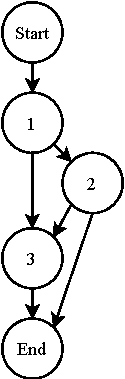
\includegraphics[height=1.5in]{img/Background/control-flow-graph.pdf}
    \label{fig:background_control_flow_graph_image}
    \end{minipage}
&
\begin{minipage}[c]{0.45\textwidth}
\centering
\begin{lstlisting}[language=Python, label=lst:background_control_flow_graph_listing]
def function(a,b):
    if a < b: # (1)
        if b < 10: #(2)
            a = a + b
        else:
            return b #(end)
    a = a * 2 #(3)
    return a #(end)
\end{lstlisting}
\end{minipage}
\end{tabular}
\caption[Control-flow graph visualisation for a code sample]{Control-flow graph visualisation for a code sample. The graph has 6 edges, 5 nodes and one connected component. The cyclomatic complexity is 3. }
\label{fig:background_control_flow_graph}
\end{figure}

The cyclomatic complexity on a control-flow graph as the number of linearly independent execution paths is defined as:
\begin{equation}\label{eq:cyclomatic_complexity}
M = E - N + 2P
\end{equation}

$E$ is the number of edges, $N$ the number of nodes and $P$ the number of connected components.  A connected graph is a subgraph, in which all nodes are connected to each other by a path. Following this definition, the cyclomatic complexity can be calculated. Figure \ref{fig:background_control_flow_graph} shows a visualisation of a sample python function. The control-flow graph has six edges, five nodes and is one connected component. Using equation \ref{eq:cyclomatic_complexity}, the cyclomatic complexity is 3.

MacCabe recommends limiting the cyclomatic complexity to 10. NIST confirms this recommendation in TODO. A lower cyclomatic complexity improves testability since the complexity represents the number of execution paths that need to be tested. Therefore, $M$ is the upper bound for the number of test cases for full branch coverage. 
Furthermore, studies suggest a positive correlation between cyclomatic complexity and defects in functions. TODO source
Software that has to comply to safety standards like ISO 26262 (for electronics in automobiles) or IEC 62304 (for medical devices) are mandated to have a low cyclomatic complexity\cite{isotc_22sc_32_iso_2018, isotisotc_210_iec_2006c_210}.

Although cyclomatic complexity is used throughout the industry, several shortcomings are under critique. First, complexity from data flow is ignored. Working with a larger number of variables and operations, the code becomes more complex, but the cyclomatic complexity does not take this into account. Second, nested code structures are not considered by the metric, although it adds additional difficulty for understanding. TODO source as Halstead critique.

\subsection{Halstead Complexity Measures}
Maurice Halstead introduced the Halstead complexity measures (HCM) in 1977\cite{halstead1977elements}. Halstead approached the complexity measure with an empirical approach by defining observable and measurable properties and put them into relations.

The measurable properties are operators and operands. Operators are symbols in expressions like an addition, subtraction or multiplication symbol. Operands are the values and variables that are manipulated by the operators. 

The sum and number of distinc operators and operands are counted as:
\begin{itemize}
    \item $\eta_1$ as the number of distinct operators 
    \item $\eta_2$ as the number of distinct operands
    \item $N_1$ is the sum of all operators
    \item $N_2$ is the sum of all operands  
\end{itemize}

From these base properties, Halstead derrived additional properties:
\begin{itemize}
    \item Program vocabulary size:
    \begin{displaymath}
        \eta = \eta_1 + \eta_2
    \end{displaymath}
    \item Program length as the sum of all operators and operands:
    \begin{displaymath}
        N = N_1 + N_2
    \end{displaymath}
    \item The volume of a program in terms of program length and program vocabulary is defined as: 
    \begin{displaymath}
        V = N * \log_2{\eta}
    \end{displaymath}
\end{itemize}

Based on those properties, code metrics can be calculated. 
First, the difficulty of understanding a program is calculated as:
\begin{displaymath}
    D = \frac{\eta_1}{2} * \frac{N_2}{\eta2}
\end{displaymath}
The major contributors to difficulty are the number of distinct operators $\eta_1$ and the sum of all operands $N_2$.

Second, the combination of difficulty and volume is the required effort for understanding or changing code follows:
\begin{displaymath}
    E = D * V
\end{displaymath}

Third, the effort for changes translates into real time following the relation:
\begin{displaymath}
    T = \frac{E}{18}s.
\end{displaymath}

Last, the number of bugs correlates with the following relation TODO cite: A survey on metric of software complexity:
\begin{displaymath}
    B = \frac{V}{3000}
\end{displaymath}

HCM focus on the complexity introduced by data manipulation but ignores complexity from the control-flow. Since the cyclomatic complexity focus on the control-flow complexity but not on the data-flow complexity, it is practical to use both together to supplement each drawback (TODO source: A survey on metric of software complexity
). Additionally, the correlation with the number of bugs is based on the programmer's skill estimation with a fixed value of 3000. Since this varies between projects, such an experiential and fixed number is doubtable (TODO source as before).

\subsection{Software Maintainability Index}
The software maintainability index was developed by Dan Coleman and Paul Oman in 1994. 16 HP engineers evaluated 16 software systems and scored it in a range from 0 to 100, with 100 representing best maintainability\cite{coleman_using_1994}. 
Following a regression analysis, they identified the following equation to match the maintainability of the evaluated systems:
\begin{displaymath}
MI = 171 - 5.2 *\ln{\overline{V}} - 0.23 * \overline{M} - 16.2 * \ln{\overline{LOC}} + 50 * \sin{\sqrt{2.4 * C}}
\end{displaymath}
$\overline{V}$ is the average Halstead Volume, $\overline{M}$ the average cyclic complexity, $LOC$ the lines of code and $C$ as fraction of comments.

The software maintainability index was defined many years ago with a limited sample size of developers and projects. Additionally, programming languages have changed significantly over time. A study by Sjøberg et al. suggest no correlation between the software maintainability index and actual maintenance effort in a controlled environment\cite{sjoberg_questioning_nodate}. Although the study only analysis four software projects and lacks generalisation, they find a strong anti-correlation with different maintainability metrics. Only the code size seems to correlate with the actual maintainability. The former seems to be consistent with a systematic review on software maintainability predictions and metrics by Riaz et. al\cite{riaz_systematic_2009}.


\section{Tools for Code Quality Analysis}\label{sec:tool_comparison}
It is good practice to use static code analysis tools to improve code quality. A static code analysis examines a program by analysing an abstract syntax tree, the control or data flow, a pointer analysis or an abstract (approximated) execution. In comparison to dynamic analysis, the code is not executed. The result of static analysis can be based on approximations, so there might be false-positive results. An expert has to examine the result and correct results if necessary\cite{prahofer_static_2017}.

Besides the use of static code analysis for compiler and optimisations, it is also helpful for analysing the code quality. Different categories of code quality-related principles can be analysed:
\begin{description}
    \item[Code Guidelines:] A static code analysis can ensure compliance to structural, naming and formatting code guidelines. 
    \item[Standard Compliance:] A requirement for a software may be compliance to an industry-standard like IEC 61508 or ISO 26262 \cite{noauthor_iec_2010,isotc_22sc_32_iso_2018}. Static code analysis can ensure or at least assist with the compliance.  
    \item[Code Smells:] Some code smells follow a known pattern and a static code analysis can detect those smells. Since code smells can be an indication for chaotic code, it is best if these smells are detected and removed early on.
    \item[Bug Detection:] Although bug detection with static analysis can not detect all bugs, every detected bug before a software release is important. Examples for detected bugs are unhandled expressions or concurrency issues \cite{delaitre_evaluating_2015}.
    \item[Security Vulnerability Detection:] Static code analysis tools can detect some security vulnerabilities like SQL Injection Flaws, buffer overflows and missing input validation with high confidence. Since these are some common, easy to exploit vulnerabilities, an analysis for security vulnerabilities can increase the security of the overall software \cite{wichers_source_nodate}.  
\end{description}

The following sections provide an overview of a few static code analysis tools with a focus on code quality and maintainability. We selected them based on popularity and if the projects are still maintained.

\subsection{PyLint}
PyLint is a code analysis tool for the Python programming language. It is open-source and licensed under the GNU General Public License v2.0 and available for all common platforms. PyLint can be executed as a standalone program or can be integrated into common IDEs like Eclipse. A continuous integration pipeline may include PyLint as well to ensure an analysis on every build.

With PyLint, the developer can make sure the code complies to the PEP8 (TODO) style guide for python coding. This includes name formatting, line length and more. It does not calculate a metric for the code but instead warns about violated principles. Additionally, PyLint can detect common errors like missing import statements that may cause the program to crash at the start or later at runtime. To support refactoring, PyLint can detect duplicated code and will suggest refactoring the code.

PyLint can be configured to ignore some checks and to disable specific rules. To expand the ruleset, a developer can write a "checker", an algorithm to check for a specific rule. The algorithm can analyse the raw file content, a token stream of the source code or an AST representation. The checker can raise a rule violation by providing the location information and the problem type to the PyLint framework and it will be included in the PyLint analysis report.

\subsection{PMD Source Code Analyzer Project}
PMD is an "extensible cross-language static code analyser" for Java, JavaScript and more. As an open-source project, it is licensed under a BSD-style license and is available for macOS, Linux and Windows-based systems. It integrates into build systems like Maven and Gradle as well as into common IDEs like Eclipse and IntelliJ. PMD can run as part of a continuous integration pipeline and is included in the automated code review tool Codacy (see TODO).

Depending on the target language, PMD supports different rules. For Java, PMD has ruled in the following categories:
\begin{description}
    \item[Best practices:] Best practices include rules like one declaration per line or using a logger instead of a \textit{System.out.print()} in production systems.  
    \item[Coding Style and Design] Several rules to improve the readability of the code like naming conventions, ordering of declarations and design problems like a violation of the law of Demeter, Cyclomatic complexity calculation and detection of god classes.
    \item[Multihtreading: ]  Rules to mainly prevent the use of not thread-safe objects or methods. Due to the nature of multi-threading and unpredictable scheduling of threads, problems like unpredictable values of variables or deadlocks may occur. Since they may not occur in every execution, they are hard to spot and to debug. Consequently, warnings of using non-thread-safe code may save hours of debugging.
    \item[Performance: ] These rules flag known operations that have hidden performance implications. For example, string concatenation with the plus operator in Java causes the Java Virtual Machine to create an internal String buffer. This can slow down the program execution if numerous String concatenations are performed.
    \item[Security:] Security-wise, PMD only checks for hardcoded values for cryptographic operations like keys and initialisation vectors.
    \item[Error Prone Code: ] PMD checks for several known code structures that will or may cause a bug at execution. Some rules are part of the clean code principles described in \ref{sec:clean_code} and some rules are specific to the target language.
\end{description}

A user can expand the PMD ruleset in two ways: A XPath expression can be specified and will be validated against the AST by the PMD framework. For more control, it is possible to write a Java-based plugin that implements a custom AST traverser. The latter allows for more sophisticated rules and checks.

\subsection{Codacy}
Codacy is a software to "automate your code quality" (TODO source) for more than 30 programming languages. It is available as a cloud-based subscription service with a free tier for open-source projects and a self-host option for enterprise customers.  Codacy runs as cloud software and a user can connect a GitHub, GitLab or Bitbucket repository that will be scanned automatically on every push or trigger a scan of local files with a command-line program. Additionally, a badge can be added to the readme page to show off the analysis results.

Codacy can be seen as a platform that runs multiple different "analysis engines". These analysis engines combine multiple tools depending on the language. For Python, Codacy uses  PyLint, Bandit (a scanner for security issues) and a metric plugin.
Due to the licensing of those analysis engines, the engines are open-sourced, whereas the Codacy platform is proprietary.

Depending on the language, Codacy supports scanning for common security and maintainability issues. The later is faced with scanning for Code Standardization, Test Coverage and Code Smells to reduce technical debt.

Codacy allows customisation by disabling certain rules and changing rule parameters like the pattern to fit the rules to the project. 

\subsection{Sonarqube}
Sonarqube is an analysis tool to maintain high code quality and security. It supports 15 programming languages in the open-source version licensed under the GNU Lesser General Public License, Version 3.0. In the Developer Edition, Sonarqube supports 22 languages and 27 languages in the enterprise edition. Sonarqube is a self-hostable server application with a SonarScanner client module that can be integrated into build pipelines like Gradle and Maven as well as a command-line tool for other build pipelines. The SonarScanner reports the result to the server, that serves a website to review the results. With the Developer Edition, branch and pull request analysis are possible and a pull request will be annotated with the analysis results.

For Python, Sonarqube offers more than 170 rules. These rules are in the following categories:
\begin{description}
    \item[Code Smells:] Code Smells like duplicated String literals are flagged with four different levels of severity (from higher to lower severity): Blocker, Critical, Major, Minor. Explanations and examples are accessible for the developer to understand and fix the issue. The analysis is more in-depth than AST-based solutions since it additionally uses control and data-flow analysis.
    \item[Bug:] Multiple rules cover bugs that would definitively result in a runtime exception and program termination. As an example, calling a function with the wrong number of arguments will be flagged with the highest severity, since it will raise a TypeError during runtime. Although programmers may notice issues like this during coding and testing, the issue can remain hidden if it only triggers a special execution path of the system.
    \item[Security Hotspot: ] The Security Hotspot analysis unfolds pieces of code that may be a real vulnerability and requires a human review. The scanning has a hotspot detection for seven out of the OWASP Top Ten Web Application security risks (TODO src). A flagged hotspot contains a detailed explanation of the reason for being flagged and a guide on how to review this hotspot. The recommendation to double-check a piece of code can help to prevent a security vulnerability from being deployed to production.
    \item[Security Vulnerabilities: ]  A security vulnerabilities analysis reveal code that is at risk of being exploited and has to be fixed immediately. Especially misconfiguration of cryptographic libraries can be revealed easily and future damage prevented.   
\end{description}

Additionally, Sonarqube offers several metrics like test coverage and a custom derivate of Cyclomatic Complexity named Cognitive Complexity\cite{campbell2018cognitive}. The authors see several shortcomings in the original Cyclomatic Complexity model:
\begin{itemize}
    \item Parts of code with the same Cyclomatic Complexity do not necessarily represent an equal difficulty for maintenance.
    \item  Cyclomatic Complexity does not include modern language features like try/catch and lambdas. Therefore, the score can not be accurate.
    \item Cyclomatic Complexity lacks useability on a class or module level. Since the minimum complexity of a method is one and a high aggregated Cyclomatic Complexity for a class is measured for small classes with complex methods or large classes with low complexity per method (e.g. a domain class with just getter/setter).
\end{itemize}
Cognitive Complexity addresses these points, especially the incorporation of modern language features and meaningfulness on class and module level.

The calculation is based on three rules\cite{campbell2018cognitive}:
\begin{description}
    \item[Ignore Shorthand Structures]: Method calls condense multiple statements into one easy to understand the statement. Therefore, method calls as shorthand are ignored for the score. Similarly, shorthand structures like the null-coalescing operator reduce the Cognitive Complexity compared to an extensive null check and are therefore ignored for score calculation.
    \item[Break in the linear control flow]: A break in the expected linear control flow by loop structures and conditionals adds to Cognitive Complexity as to Cyclomatic Complexity. Additionally, Catches, Switches, sequences of logical operators, recursion and jumps also adds to Cognitive Complexity, since these structures break the linear control flow.
    \item[Nested flow-breaking strcutures]: Flow-breaking structures that are nested additionally increase the Cognitive Complexity, since it is harder to understand than non-nested structures.  
\end{description}
The method-level Cognitive Complexity score represents a relative complexity difference between methods that would have the same Cyclomatic Complexity. Furthermore, the aggregated Cognitive Complexity on a class or module level now differentiate between classes with many, simple methods and classes with a few, but complex methods. As a result, domain classes (containing mainly getters/setters) have a lower score compared to classes with complex code behaviour\cite{campbell2018cognitive}.

Developers can extend Sonarqube similarly to PMD. They can write a Java plugin that can access the AST but also a semantic model of the code. Additional, extensions can be created that provide the functionality to other extensions. The Java plugin is compiled into a .jar file and placed into the plugin dir of the Sonarqube installation. For simpler rules, XPath expressions are possible through the web interface and allow a quick extension. For instance, if developers observe bad code style during a pull request review, they can quickly write a rule to enforce this rule in all subsequent pull requests automatically.

Integration in continuous integration, manual review

Tools review for all tools that check different stuff

Single Responsible principle, Open-Closed principle



\chapter{Approach}
Approach(es) without the quantitative results (or only selected results to motivate the choices/the problems)

What has possibly failed (short)

What has worked and why

What could be possible method extensions/improvements

This section is divided into the approach for the Clean Code Analysis Plattform and the Clean Code classification.

\section{Clean Code Analysis Plattform}
The goal of the design and implementation of the Clean Code Analysis Plattform (CCAP) is a tool for software developers to improve the code quality of existing and new code. The tool accepts a directory containing source code files as input and analyses the input for snippets of improvable code quality. If the analysis classifies a code snippet as problematic, it should help the developer to improve the snippet by providing information about the problem. Ultimately, this should train the developer to spot problematic code by its own and to write clean code by default, so the number of alerts should decrease. At the same time, the overall software quality of a project increases immediately at rewriting a marked snippet and in the long term at training the developer to write code with higher quality.

In order to use the tool effectively, the design and implementation should cover the following requirements:
\begin{description}
    \item[Useability]:  The CCAP should be an easy-to-use tool. Developers shall be able to install and run the tool. The extra effort of using this tool should be small, and the developer should use the tool in his day-to-day workflow without additional friction. The developers can interpret the issue and localise the problematic code spot immediately.
    \item[Expandability]: The extension of the detected code problems should be easy. A clear defined interface for extensions is required so an extension developer would not need specific knowledge about the internal architecture of the tool. The expandability allows the desired workflow of a developer finding problematic code in an, e.g. peer-review, formalising it into an extension and sharing this extension with the team. With each iteration, the code quality of all team members would increase.
    \item[Integration]: The tool should be easy to integrate into different systems. These systems include local workflows like git pre-commits or build systems and remote continuous integration/delivery/deployment pipelines.
\end{description}
A more specific requirement is Python as an input language and the expansion language. After JavaScript, Python is the second most popular programming language 2019 according to the Github statistics (\url{https://octoverse.github.com/#top-languages}). Besides the general popularity, Python is heavily used in the scientific community for machine learning and universities for teaching programming. These groups are part of the potential target audience, and students in specific can benefit from automated reporting of low-quality source code.

\subsection{Architecture}
The CCAP architecture is divided into a static part and two extension possibilities: An extension with analysis plugins adds more rules that are validated by the system. Adding an output plugin allows specifying the output format to fit custom workflow needs.
The static part consists of four components: A core component to act as an orchestration unit, a  component for handling the source code input and a component for handling the analysis plugins as well as output plugins. The design follows the requirements and goals for the platform. 
(TODO: High-level architecture schematic diagram)

The core component contains the main function and handles argument validation and parsing. Furthermore, it orchestrates other components by initialising and executing those. This process is divided into the argument parsing, initialisation and execution phase:
In the argument parsing phase, the command line arguments are parsed and validated. It validates the existence of the required input directory argument and the optional plugin path configuration for the analysis plugins and the output plugins. Additionally, the logging level and the output format can be defined. The latter determines, which output plugin will be used, although the existence of the specified plugin is not validated in this phase. A parsing or validation error will cause a program termination without further processing.
The initialisation phase instantiates all components and the analysis plugin handler will scan the specified directories for plugins and keeps an index of all found plugins in memory. The output plugin manager scans for an output plugin, that satisfies the specified argument. If no plugin matches the output argument, the program will terminate with a one exit code and a failure message to indicate the problem.
In the execution phase, the input handling component scans the input directory for files ending with \textit{.py} and parses the source code into an Abstract Syntax Tree (AST) per file. In the next step, the core passes the parsed data to the analysis plugin handler. The latter will execute all plugins for all files and collects the results. Afterwards, the core component calls the output plugin component to output the results. If no exceptions occur during the execution phase, the program will be terminated with a zero exit code indicating the successful run.

The input component scans the given input directory for all Python source code files and parse the source code into an AST. 
For scanning the input directory, an algorithm will walk recursively over all folders and files. The detection of Python source code files is based on the file ending \textit{.py}. The algorithm will return a list of file paths and the corresponding file content. 
Next, the AST parser is called and will add a parsed AST object to the list besides the file path and content. This list will be passed to the analysis plugins by the analysis plugin handler.  An alternative approach would be to not read and parse the code in the input component, but instead, let the plugins read and parse the file content if needed. With many files to scan, the latter approach would have a lower memory footprint since the file content and the AST will not be held in memory. Consequently, every analysis plugin has to perform an expensive read operation from disk and the performance scales with the number of files and the number of analysis plugins. 
If the input component reads all files, the information is held in the main memory and the performance only scales with the number of files. Since the files are text-based, the number of files needed to exceed the main memory is expected to be high enough to fit most projects.

The analysis plugin handler manages all analysis plugins. This component finds all plugins, executes the plugin and collects the reported results.
During the initialisation phase of the core component, the analysis plugin handler will scan the plugin directory for all Python files. It imports all Python files and scans those for classes, that inherit from an abstract \textit{AbstractAnalysisPlugin} class. The abstract class defines all methods that need to be implemented in the concrete plugin subclass. The analysis plugin handler instantiates all found classes.
During the core execution phase, the core receives a list with the file name, file content and the parsed AST. All plugins are called on a specific entry point method that is defined in \textit{AbstractAnalysisPlugin} with the aforementioned list. The plugin will return an instance of \textit{AnalysisReport} with the plugins metadata and a collection of problems. The report is collected for every plugin into an \textit{FullReport}. Additionally, the report contains information about the overall plugin execution time and run arguments. After all plugins have been executed for all files, the analysis plugin handler returns the \textit{FullReport} to the core component.

The last component in the execution chain is the output plugin handler that will pass the \textit{FullReport} to the specified output plugin. It implements the same algorithm as the analysis plugin handler to find all plugins that inherit from \textit{AbstractOutputPlugin}. Instead of keeping track of all plugins, only the plugin that corresponds to the output format argument is instantiated. The output plugin has an entry point as defined in \textit{AbstractOutputPlugin}  that is called with all the collected results.

\subsubsection{Analysis Plugins}\label{sec:analysis_plugins}
Analysis plugins provide the easy extendability of the platform by developers. All users of the tool can expand the set of problems it can detect by implementing a plugin Python and placing it into the plugin directory of the tool. In order to be compatible with the core components, a plugin has to be a class that inherits from the \textit{AbstractAnalysisPlugin} class. Firstly, the abstract class introduces a class member variable \textit{metadata} of the class \textit{PluginMetaData}. A concrete plugin class sets this class member in the constructor to provide a plugin name, author and optional website. This metadata is used in the output to show more information about the plugin that reported a problem. Secondly, \textit{AbstractAnalysisPlugin} specifies a \textit{do\_analysis} method that serves as a entry point that the platform will call. It accepts a list of \textit{ParsedSourceFile} objects that contains the file path, the file content and the corresponding AST for all input files. With this information, the plugin can implement any logic to detect problems. 
For example, the plugin can traverse the AST to look for specific node types, it can use a tokeniser on the content of the files and analyse the token stream or it can run sophisticated machine learning algorithms on the source code.
The plugin can even import third-party libraries, although they have to be installed by the user on the system. After detecting all problems, the plugin returns an \textit{AnalysisReport}. The report contains the plugins metadata and a list of found problems. These problems are instances of a problem class inheriting from \textit{AbstractAnalysisProblem}. The abstract class expects a file path and line number as constructor arguments and requires the plugin developer to override the problem name and description (see \Cref{lst:lst:return_none_problem_override} for an example). The problem name and description will be shown in the final output and should follow the following guidelines:


\begin{lstlisting}[language=Python, label=lst:return_none_problem_override, caption={Example for overwriting the \textit{AbstractAnalysisProblem} with a concete implmentation. The problem name and description are overwritten.}]
class ReturnNoneProblem(AbstractAnalysisProblem):
    def __init__(self, file_path, line_number):
        self.name = "Returned None"
        self.description = "Returning None is dangerous since the caller has to check for None. Otherwise, a runtime exception may occur."
        super().__init__(file_path, line_number)
\end{lstlisting}

\begin{itemize}
    \item Have a proper name that allows the experienced developer to recognise the problem quickly.
    \item Explain what code construct is problematic.
    \item Give reasons why this code is seen as problematic.
    \item Show guidance and examples on how to fix the problem and improve the code.
\end{itemize}
Although it is possible to use one plugin for multiple, different problem types, having one plugin for one problem type helps to reuse and share the plugin. Additionally, it can be disabled easily by removing the plugin from the plugin folder.

\paragraph{Steps to create an analysis plugin}
In order to expand the CCAP with an analysis plugin, the following steps are required for a developer:
\begin{enumerate}
    \item Create a \textit{.py} file with a class inheriting from \textit{AbstractAnalysisPlugin}.
    \item Instanziate \textit{PluginMetaData} and assign it to the metadata member.
    \item Define a problem class inheriting from \textit{AbstractAnalysisProblem} and set the problem name and description following the guidelines above.
    \item Implement the \textit{do\_analysis} method with a \textit{ParsedSourceFile} parameter. Return an \textit{AnalysisReport} instance with all found problems.
    \item Place the \textit{.py} file into the analysis plugin directory of the tool.
\end{enumerate}
Whereas these are the minimum required steps to implement the plugin, the developer is free to add additional methods, classes or import libraries as necessary.
Furthermore, it is advisable to implement several tests to ensure the plugins correctness. CCAP uses pytest \footnote{\url{https://docs.pytest.org/en/stable/}} for testing, implementing a test is as easy as writing a function with a \enquote{test\_} prefix and running the \textit{pytest} command. The plugin can be tested by simulating a call from the CCAP core with a mocked \textit{ParsedSourceFile}. 

\paragraph{Return None Plugin}
A rather simple analysis plugin demonstrates the capabilities of the CCAP: The Return None Plugin scans the source code for functions that return the None value. Returning None may result in runtime exceptions if the function caller does not expect and handle a potential None return. Although the None can be returned directly or as a value of the returning variable, this plugin only focus on the explicit \textit{return None} statement to showcase the options for the developer to analyse the source code.

Detecting \textit{return None} is possible in multiple ways. The following shows the possibilities for developer to implement such a detector:
\begin{description}
    \item[Regular Expression]: In the \textit{do\_analysis} method, a developer has access to the source code as a string. Therefore, it is straitforward to use a regular expression to detect a \textit{return None} statement.
    \begin{lstlisting}[language=Python]
import re
matches = re.finditer(r"return None", source_file.content, re.MULTILINE | re.DOTALL) \end{lstlisting}
    Since the regex library only returns the start and end index of matches, these have to be converted to line numbers. Afterwards a \textit{ReturnNullProblem} instance can be created for every match and added to the \textit{AnalysisReport} for this plugin.

    This approach uses regular expressions to match patterns in a string without utilising the structures of the code. It is a simple but powerful way and most developers are familiar with regular expression. On the flip-side, source code may have various ways syntactic ways to express a semantic. Consequently, the regular expressions have to be designed carefully to cover all variations. For instance, it is possible to encounter a doubled whitespace, that would break the aforementioned regular expression. Additionally, regular expressions do not operate on the structure of the code; therefore, they can not detect high-level patterns on the code structure.
    \item[Tokenisation]: The process of dividing a character stream into a sequence of tokens is called tokenisation (also known as lexical analysis). With the Python tokeniser, a token can contain multiple characters and has a token type like name, operator or indentation. A token sequence provides more information about the code structure that can be used to detect problematic patterns. 
    A token sequence for a \textit{return None} statement would be the following: 
    \begin{lstlisting}
    [...(type: NAME, value: return), (type: NAME, value: None)...]
    \end{lstlisting}
    A simple algorithm would scan the sequence for two subsequent name tokens with the values "return" and "None". The abstraction level of a token sequence is higher than of a character sequence. Since the whitespace between "return" and "None" provide no semantic meaning, it is removed on this abstraction level. Whereas the regular expression based approach would have to deal with problems as the doubled whitespace, the token-based approach profits from the higher abstraction level and can access meaningful tokens directly.
    \item[Abstract Syntax Tree]: After tokenisation, a parser takes the token stream and prases it into a hierarchical data structure like an Abstract Syntax Tree. With an AST the code is represented structurally and it is possible to traverse the tree following the structure of the code. The AST consists of nodes with different type and children, for example, a node representing an if statement. It is possible to access the condition and the body of the if statement as descendant nodes in the AST. Analysing an AST allows a higher abstraction level then analysing the token string since the code structure is represented. Therefore, more abstract rules that analyse the code structure are possible.

    To detect a \textit{return None} statement in the abstract syntax tree, an algorithm would traverse all AST nodes looking for a return-typed node. If found, the value descendant contains the statement part after the return keyword. A \textit{None} value would be represented as a node of type constant or name constant (depending on the parser version). The value descendant of the constant node may then be checked for equality to \textit{None}. All AST nodes contain the corresponding line number, that are necessary for creating a problem message. See \Cref{lst:return_none_detection_algorithm} for a Python implementation. 


    Analysing the AST is best for problems in the code structure since the AST represents the code structure in a well-defined, traversable data structure. Although simpler patterns like the \textit{return None} could be detected using regular expressions, a detection on AST level allows detecting the semantic meaning instead of the syntactic representation of a problem. For more complex problems, it is inevitable to use the AST most of the time.
\end{description}

\begin{minipage}[c]{\linewidth}
    \begin{lstlisting}[language=Python, label=lst:return_none_detection_algorithm, caption={Detecting RETURN NONE problems by analsing the AST data structure.}]
    for node in ast.walk(a.ast):
        if isinstance(node, ast.Return):
            return_value = node.value
            if isinstance(return_value, ast.Constant) or isinstance(return_value, ast.NameConstant):
                if return_value.value is None:
                    problems.append(ReturnNullProblem(a.file_path, return_value.lineno))\end{lstlisting}
    \end{minipage}

This implementation covers only the simple case, in which \textit{return None} is written explicitly. Of course, several modifications are possible, that would not be detected by this plugin and would require more sophisticated algorithms. Evaluating, if machine learning models trained on this simple rule can also detect such modifications is part of the second part in \hyperref[rq:3]{RQ3}.

Since detection alone is not a great help for the user, a useful description of the problem is necessary. 
As described in \Cref{sec:background:returning_none_and_error_handling}, there are some alternatives to returning none. If returning \texttt{None} due to an error, it is better to raise an exception and provoke an explicit error handling, which prevents runtime errors. If the standard return type is a collection, an empty list is more appropriate, since the function caller will most likely write the logic for an unknown amount of list items. However, if the standard return type is a single object, it is not apparent what to return. With PEP484 (TODO source), an optional type was introduced for type hints in Python 3. Using a static type checker for Python like mypy (TODO source) outputs a warning if a developer forgets to check an optional for not being none. 

\paragraph{Condition with Comparison}\label{sec:condition_comparison}
The second plugin detects a direct comparison in a conditional statement. For better readability and understandability, it is suggested to use a function call with an appropriate name that evaluates to true or false. This function call allows a natural reading of the conditional statement without deciphering the meaning of the boolean logic.

An if-statement consists of a condition and body part. If the condition evaluates to true, the body is executed. For the condition, any logical expression will be evaluated. A simple algorithm would take the AST, search for if nodes and check if the condition part is a compare node.
However, negation and logic AND/OR would not be detected by the simple approach. Consequently, a recursive algorithm has to follow logic operators and checks the expressions for comparison nodes. The simple approach does not provide value for the CCAP but we use if for the machine learning evaluation with the problem type name CONDITION COMPARISON SIMPLE.

Following these considerations, an advanced algorithm would scan for if nodes in the AST. The conditional part as a boolean expression is evaluated in a recursive function that returns true if a direct comparison is made anywhere in a boolean expression.
The conditional part can be a boolean operation (like AND/OR) or a unary operator (like NOT).  In these cases, the recursive function will be called again with the respective expressions. If the conditional part is neither a boolean operation nor a unary operator, a true is returned if the conditional part is not a method call. The last case would be the base case in the recursion. \Cref{lst:condition_coparison} shows the Python implementation of the recursion.
\begin{lstlisting}[language=Python, label=lst:condition_coparison, caption={Recursive function to analyse an if statement for direct comparisons. Since a condition should contain a method call, the function returns False if this is not the case.}]
def _check_if_direct_comparison(self, node):
    if isinstance(node, ast.BoolOp):
        violated = False
        #check all expressions of the boolean operator
        for value in node.values:
            if self._check_if_direct_comparison(value):
                violated = True
        return violated
    elif isinstance(node, ast.UnaryOp):
        return self._check_if_direct_comparison(node.operand)

    return not isinstance(node, ast.Call)\end{lstlisting}

\subsubsection{Output Plugins}
With output plugins, CCAP adds additional flexibility towards the output format. Depending on environmental requirements, the output can be adapted with custom logic by defining an output plugin. For instance, running the tool locally could write the results to the standard output in a human-readable way or create a formatted HTML file to be displayed in the browser. A machine-readable JSON output may be preferred when running inside an automated workflow.

Output plugins follow similar concepts as analysis plugins. A plugin class inherits from \textit{AbstractOutputPlugin}. The abstract class introduces the metadata member of the \textit{PluginMetaData} class to encapsulate plugin name and author information. Additionally, a second member variable \textit{output\_format} has to be defined with a short abbreviation for the output format. This field is used by the output plugin handler to select the output plugin by the run arguments. Consequently, it should be unique; otherwise, the first found plugin with a matching \textit{output\_format} field is selected by the output plugin handler. Therefore, using a custom prefix string is recommended.

As entry point method, the method \textit{handle\_report} has to be implemented. The method provides an instance of \textit{FullReport} as its argument. The  \textit{report} field holds a collection of  \textit{AnalysisReport} for every analysis plugin that has been executed. With metadata and problem information, the output plugin has access to all required information to produce the desired output.

\paragraph{Steps to create an output plugin}
To expand the output capabilities of the CCAP, the following steps are, similiar to analysis plugins, required:
\begin{enumerate}
    \item Create a \textit{.py} file with a class inheriting from \textit{AbstractOutputPlugin}.
    \item Instanziate \textit{PluginMetaData} and assign it to the metadata member.
    \item Set the \textit{output\_format} field with a unique abbreviation for this output format. Since it should be unique, a custom prefix prevents a name collision with preexisting plugins.
    \item Implement the \textit{handle\_report} method with a \textit{ParsedSourceFile} parameter. 
    \item Place the \textit{.py} file into the output plugin directory of the tool.
\end{enumerate}

\paragraph{Standard Output Plugin}
The Standard Output Plugin writes the formatted output to the stdout stream. It is enabled if no output plugin is explicitly specified. 

The output is divided into a general part and the problem list. The former contains the input path, all executed plugins, a total runtime and a summary field with the numbers of problems in total. The latter displays the list with problems, grouped by analysis plugin.  
For each problem, the problem name, file path, line number and description is printed. A colon separates the file path and line number. Some terminals parse the path and line number so that a user can click the path and it opens the default editor with the cursor in the correct line. Sample output is shown in \Cref{lst:stdout}.

\begin{minipage}[c]{\linewidth}
\begin{lstlisting}[ columns=fullflexible, label=lst:stdout]
Analysis Report on /Users/d064518/MA_CleanCodeAnalyser/test_programs.
Analyse Plugins: Condition Method Call Plugin, Simple Condition Method Call Plugin, Return None (Null) Plugin, Sample Plugin.
Total time: None
Summary: Found 16 problem(s)
    ----------------------------------------
PROBLEMS:
    PLUGIN NAME: Condition Method Call Plugin by Enrico Kaack <e.kaack@live.de>
        Found: Explicit comparison in condition in /Users/d064518/MA_CleanCodeAnalyser/test_programs/return_none.py:18
            Explicit comparisons in conditions should be replaced by method call for better readability
...
PLUGIN NAME: Return None (Null) Plugin by Enrico Kaack <e.kaack@live.de>
        Found: Returned None in /Users/d064518/MA_CleanCodeAnalyser/test_programs/return_none.py:4
            Returning None is dangerous since the caller has to check for None. Otherwise, a runtime exception may occur.
\end{lstlisting} 
\end{minipage}

\paragraph{HTML Output Plugin}
For larger projects, the Standard Output Plugin may not be sufficient to get an overview of the project or to generate a report. Therefore, the HTML Output Plugin creates a \textit{report.html} file, that can be opened in every browser and provides a cleaner overview. It has similar general data at the top as the Standard Output Plugin, but it moves the problem description into a tooltip to offer a more compact overview. See \Cref{fig:screen_html_output} for an example screenshot.

\begin{figure}
    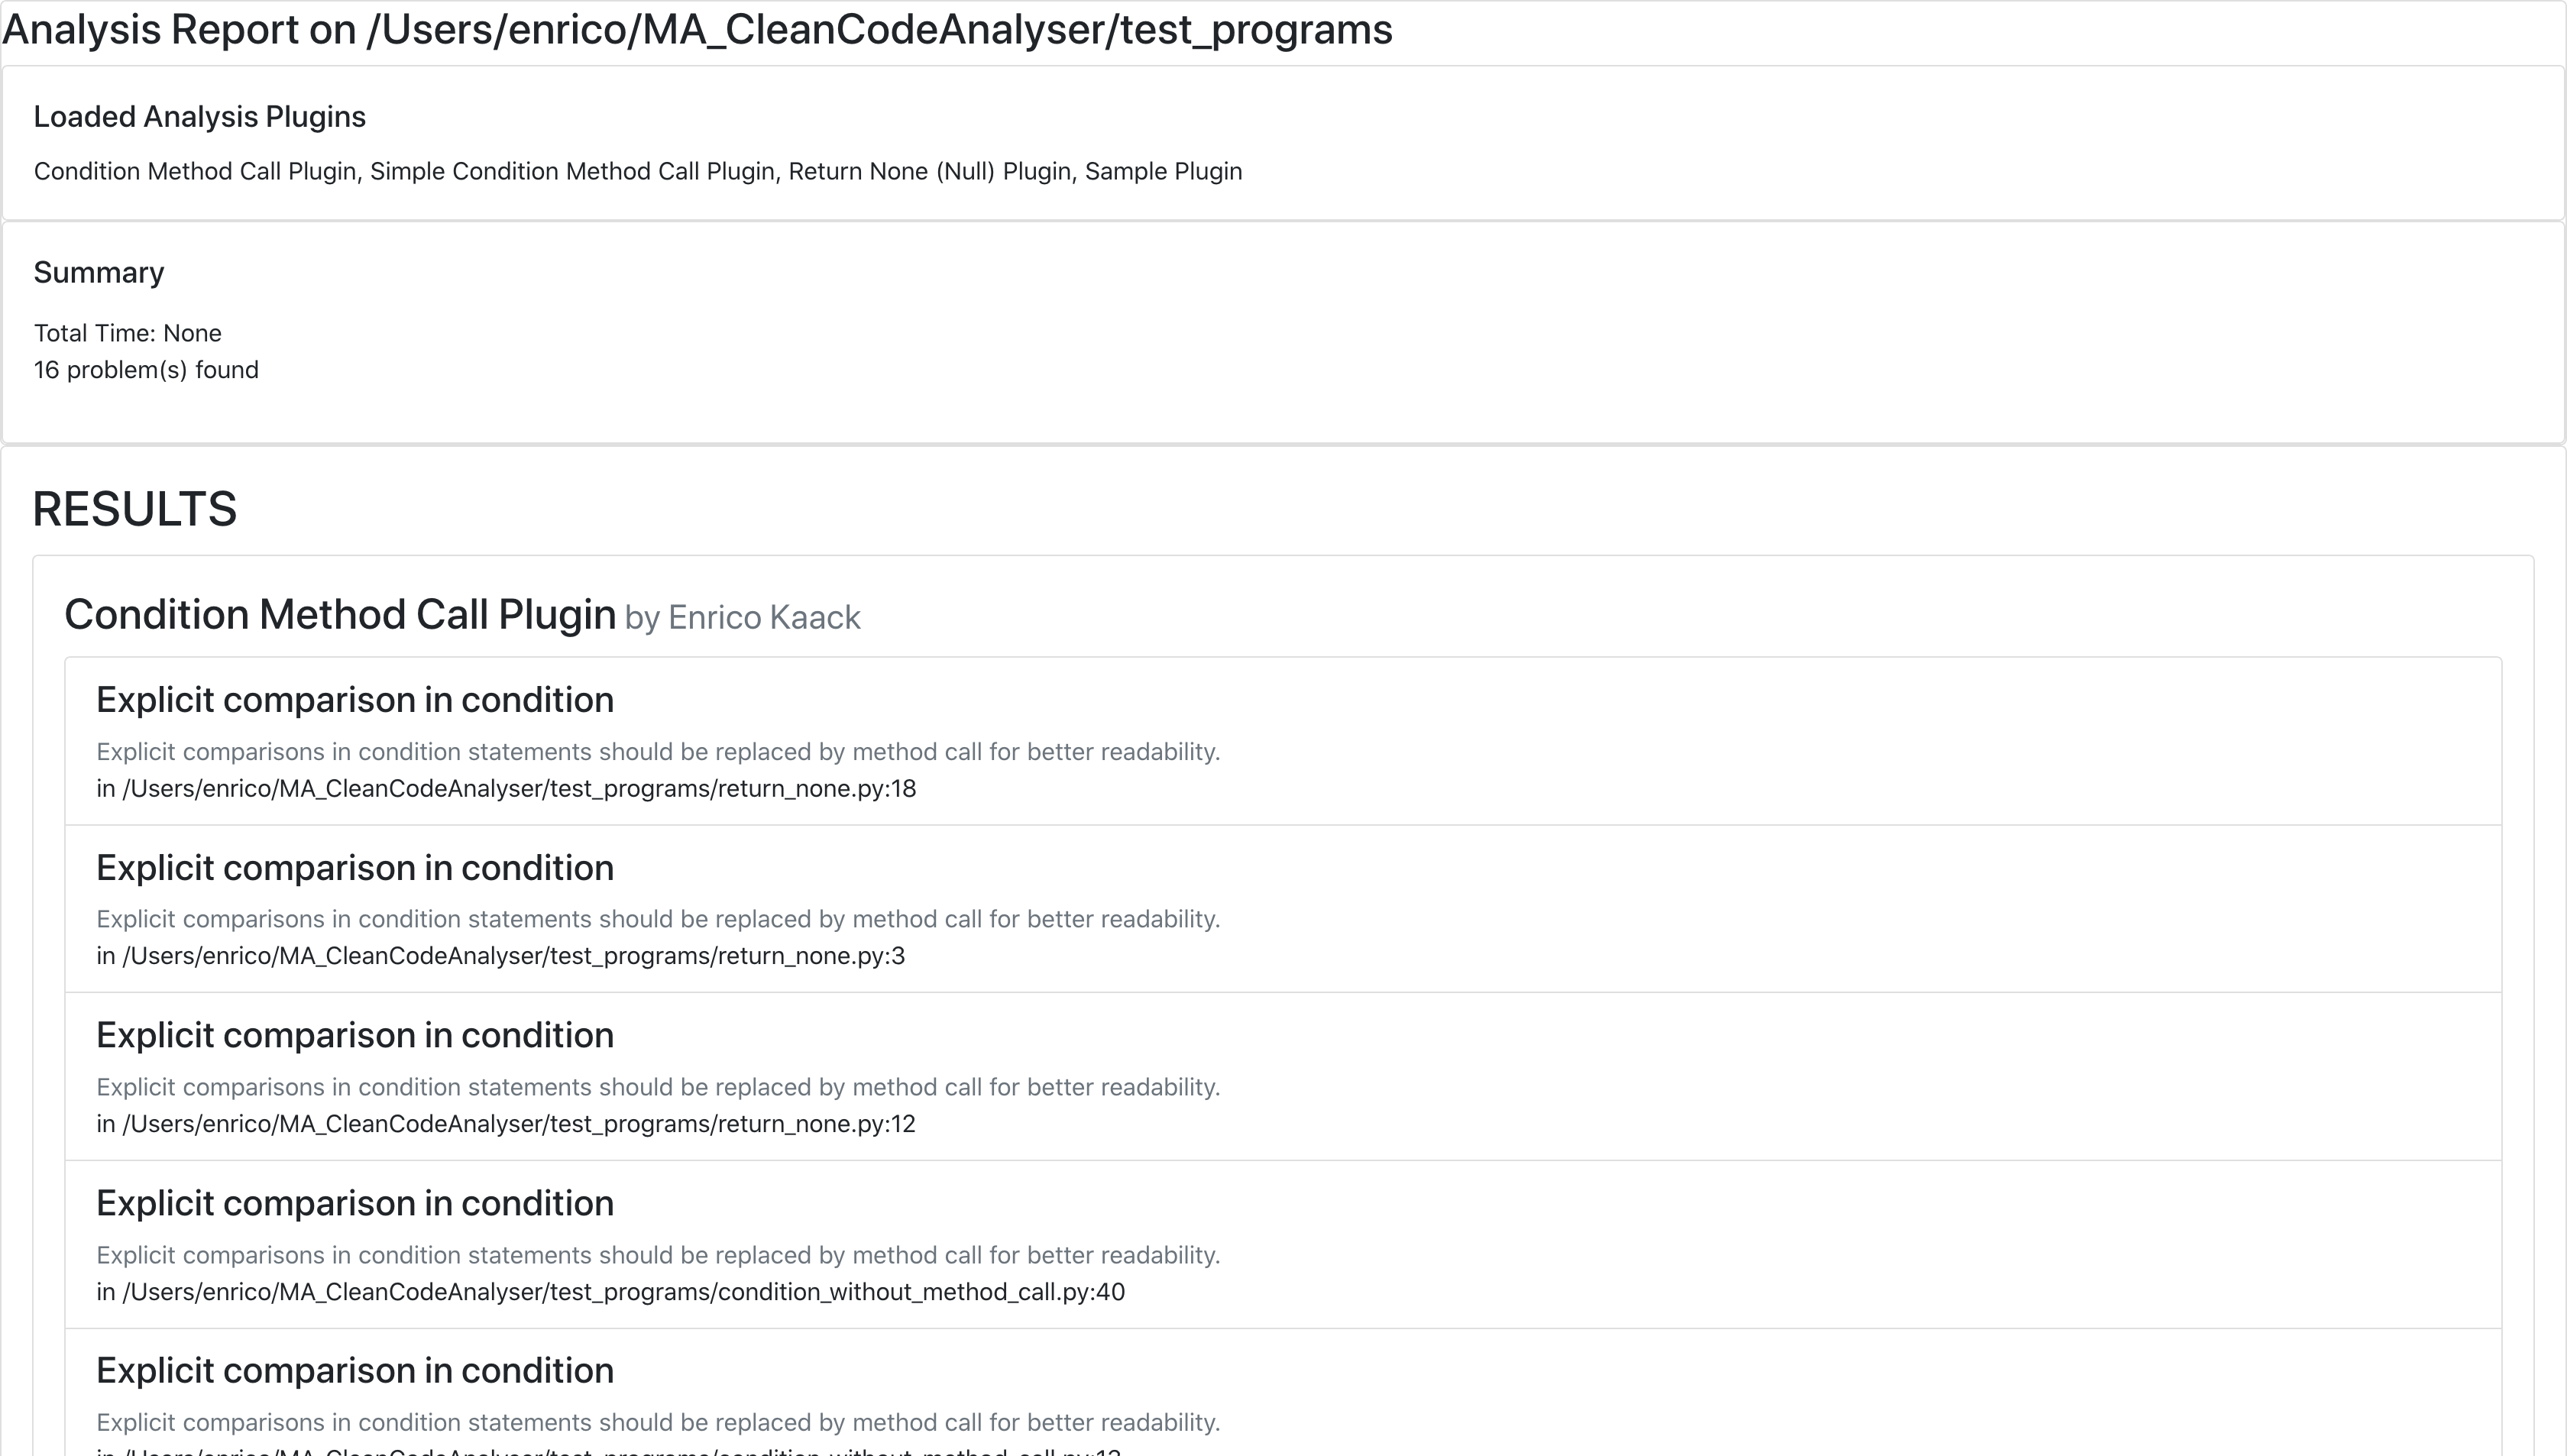
\includegraphics[width=1\textwidth]{img/CCAP/screenshot_html_output.png}
    \caption{Output of the HTML Output Plugin, displayed in a browser.}
    \label{fig:screen_html_output}
\end{figure}

\subsection{Extensions}
While the core functionality exists, extensions for the CCAP would aim for improved useability for the user. One important improvement in useability would be an IDE integration for common IDEs like Visual Studio Code. A good starting point would be the Langauge Server Protocol\footnote{\url{https://microsoft.github.io/language-server-protocol/}}. This IDE integration requires a language client as a Visual Studio Code extension and a protocol-compliant language server. The latter would wrap the CCAP and modify it slightly to process a single, changed document and return the results. Since the CCAP architecture is modular, this is possible without larger modifications. 

Another feature would be a configuration to disable specific analysis plugins, that one does not want to run on the project. With the current architecture, this would be possible by moving the analysis plugin file outside the plugin directory. A configuration with command-line parameters or with a per-project, hidden config file would have a better user experience. The latter could also be committed to the version control system, so every team member has the same configuration.
Continuing on configuration possibilities, having configuration possibilities for plugins would increase flexibility for a plugin developer. Introducing configurable warn levels like \enquote*{warning} or \enquote*{error} could help in continuous integration pipelines to decide if a build succeeds but the warnings are reported or if a build should fail because of error-level problems. Some rules could be seen as recommendations (warning level), whereas other rules would be unacceptable (error level).

Lastly, a feature to disable problem reporting for a specific code location could bring a boost in user acceptance. While some clean code rules are objective and can be measured precisely, some rules are more general recommendations that may not apply to every occurrence of this situation. For instance, the clean code guidelines generally suggest not to have more than three function arguments; it may be necessary or even inevitable to have four arguments. The CCAP should report this as a problem, but the user should be able to decide if it is acceptable. In this case, the problem type on this specific location should not be reported in the future. In the current version, the user has no way to ignore a specific problem. Consequently, over time the number of problems the user has to ignore will accumulate until the user abandons the tool since it does not provide an added value over the frustration of manually ignoring problems.

\section{Clean Code Classification}\label{chap:clean_code_classification}
In the previous chapter, we have presented a platform to check for clean code rules. This platform requires analysis plugins to detect certain problems. These handwritten rules work well on certain rules, but certain rules may require a complicated analysis of the AST, the data-flow or the inter-module dependencies. Some rules on the other hand are subjective and we do not see a way of detection those rule violations with an algorithm.
Therefore, this chapter introduces an approach to evaluate different supervised machine learning models to classify code into clean code or problematic code. Furthermore, we describe how we modify the code to test the generalisation capabilities of the models. The mentioned machine learning models include random forest classifier, support-vector-Machines, gradient boosting classifier and a recurrent neural network based on Long short-term memory units. 

The objectives are to train, evaluate and compare Source Code Snippet Classification models and to modify the input data to represent a problematic code in an unseen way.

In the following we describe the approach in detail. The strucutre follows a machine-learning typical pipeline of data collection, preprocessing, encoding, splitting and training. 

\subsection{Challenges}
\paragraph{Lack of datasets}
The most crucial components of every machine learning experiment are labeled datasets. For clean code detection, our research has shown no datasets with labeled clean code violations that could be used.
As a result, we evaluated differnent different appraoches:

\subparagraph{Solution 1:}
Related research fields like code completion often use the py150 dataset to train models~\cite{raychev2016probabilistic}. This dataset contains 150.000 python files, sourced from GitHub. For supervised classification tasks, this dataset is inadequate due to its missing labels.  

\subparagraph{Solution 2:}
Another possible data source would be git commit histories. We could scan the history for commits that fixed unclean code. The previous code could than be labeled \enquote{unclean} and the commited code would be \enquote{clean}.
Same applies to issues and referenced pull requests on GitHub.
We dismissed this approach for several reasons (see \Cref{fig:commit_messages} for an illustrative example):
\begin{enumerate}
    \item There is no annotation in neither issues descriptions nor git commit messages that would reliably tell, if the change is changing a violation of the clean code rules.
    \item Even if we would be able to find commits that improve chaotic code, we could not ensure automatically, that the commit message is correct and only the improvement is included in the commit.
    \item Searching for commits, we found several clean code improvements and refactorings of large portions of the code base in one commit. Additionally, it is often not explicitly mentioned, which rule applied for the improvement. Consequently, a training with such data could only lead to binary classification into clean code or unclean code. From a practical standpoint, it is advantagous to name the explicit rule violation and to explain how to improve.
\end{enumerate}

\begin{figure}
    \begin{subfigure}{\textwidth}
        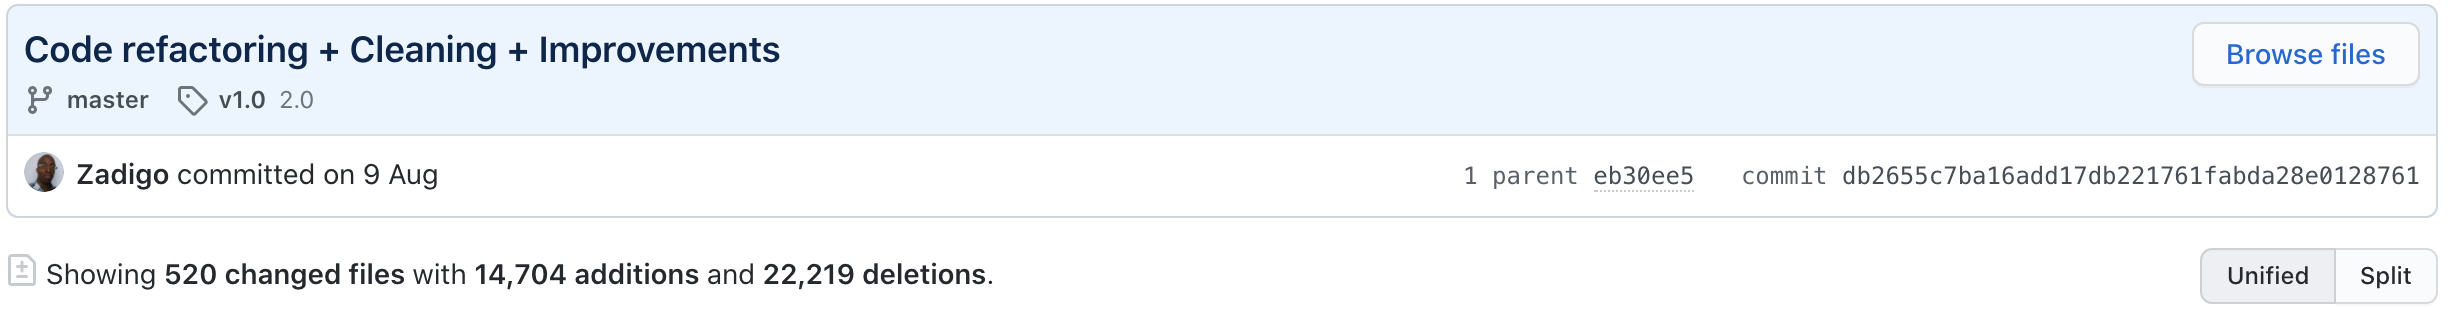
\includegraphics[width=1\linewidth]{img/ML/commit_messages/screen_1.png}
    \end{subfigure}
    \begin{subfigure}{\textwidth}
        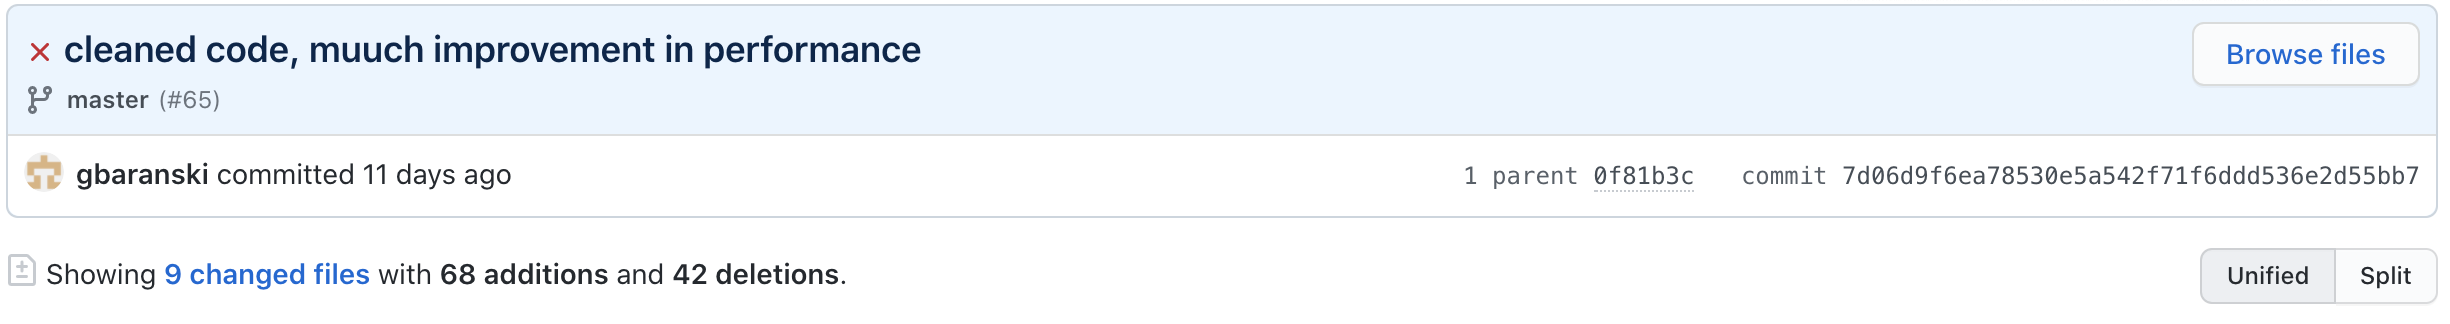
\includegraphics[width=1\linewidth]{img/ML/commit_messages/screen_2.png}
    \end{subfigure}
    \begin{subfigure}{\textwidth}
        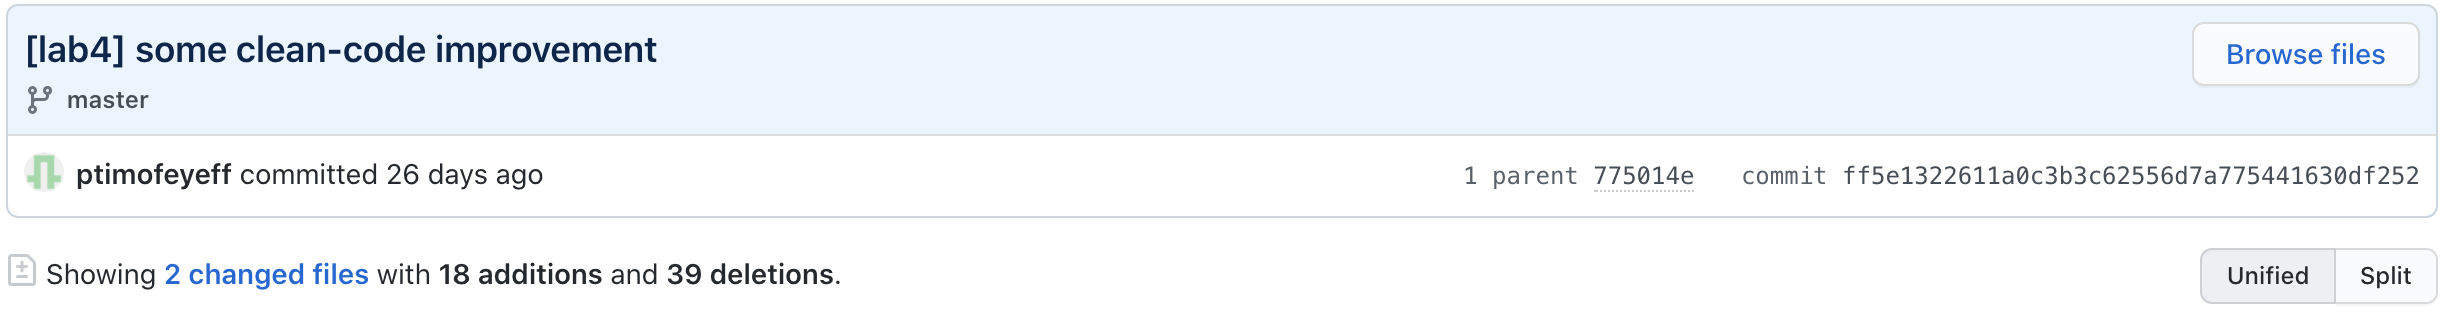
\includegraphics[width=1\linewidth]{img/ML/commit_messages/screen_3.png}
    \end{subfigure}
    \caption[Example commit messages that underline the inconsistency in commit message naming]%
    {Example commit messages from different repositories. Those examples highlight (1) the missing naming convention, (2) inclusion of additional performance improvements and (3) several edits in multiple files. Those commits are found by searching GitHub for \enquote{clean code improvements} and filtering for Python language and commits. Sources: \footnotemark[1], \footnotemark[2], \footnotemark[3]  }
    \label{fig:commit_messages}
\end{figure}
\footnotetext[1]{\url{https://github.com/Zadigo/ecommerce_template/commit/db2655c7ba16add17db221761fabda28e0128761}}
\footnotetext[2]{\url{https://github.com/gbaranski/homeflow/commit/7d06d9f6ea78530e5a542f71f6ddd536e2d55bb7}}
\footnotetext[3]{\url{https://github.com/ptimofeyeff/distributed-computing/commit/ff5e1322611a0c3b3c62556d7a775441630df252}}
\subparagraph{Solution 3:}
Although Python code is available in abundance in form of open-source projects, it is possible to manually label source code that violates clean code guidelines. 
For the following reasons, we dismissed this approach:
\begin{enumerate}
    \item Curating a hand-labeled dataset is a lot of work that takes time. 
    \item Manual labeling does not ensure correct labeling. A human can make mistakes or can subjectivly misinterpret chaotic code as clean code. The quality of the dataset could suffer and limit the machine learning models performance.
\end{enumerate}
\subparagraph{Solution 4:}
Given any amount of Python files, we could use the analysis plugins from \Cref{sec:analysis_plugins} to reliably detect violations of the corresponding rule. Based on this labeled data, we can train the classifier to detect these rules. If there would be a labeled dataset for more complex clean code rules, we could transfer the findings to these more complex rules. We choose this solution as to solve the dataset problem and train classifier, with more details given in \Cref{sec:data_encoding}. As a second step, we manipulated the input data, so the original analysis plugin could not detect the still existing problems anymore. With the second step, we show that the classifier generalise well enough to may work on complex clean code rules.

\paragraph{Inbalanced Dataset}\label{sec:inbalanced_dataset}
A second challenge is a major inbalance between the classes labeled as problematic code and clean code. For the three different problem types, RETURN NONE, CONDITION COMPARISON SIMPLE and CONDITION COMPARISON, the class distribution is shown in \Cref{tab:class_distribution_in_dataset}.



\begin{table}[]
    \begin{tabular}{@{}llll@{}}
    \toprule
    Label  & RETURN NONE & CONDITION SIMPLE & CONDITION COMPARISON \\ \midrule
    0 & 99.79\%     & 97.36\%          & 95.14\%              \\
    1 & 0.21\%      & 2.64\%           & 4.86\%               \\ \bottomrule
    \end{tabular}
    \caption{Class distribution for the train/test dataset before the split. Label [0] represents clean code and label [1] marks problematic code of the corresponding category.}
    \label{tab:class_distribution_in_dataset}
    \end{table}


\subparagraph{Solution 1:}
Due to the inbalance, we do not choose accuracy as a suitable evaluation metric, since classifiying all samples as clean code would result in a accuracy of 99.79\% for the RETURN NONE problem type. Instead, we use precision and recall as metric, with a f1 score as single, weighted metric. More details about the metrics are in \Cref{par:approach}.

\subparagraph{Solution 2:}
We will apply undersampling and oversampling techniques on the data and evalaute the difference in model performance. Undersampling removes random samples from the majority class and thus balance class labels. Oversampling replicates random samples from the minority class to balance class labels while also increasing the overall amount of data. This technique is only used on the trainings data. Since it changes the data distribution, an additional train-dev dataset is used as an additional test set to evaluate the impact of the resampling on the model performance. 

\subparagraph{Solution 3:}
Our approach of training different classifier is a solution to the data inbalance, since different classifier have a different sensitivity to data balance. 

\paragraph{SVM quadratic complexity in training}\label{sec:svm_quadratic_complexity}
The implementation of the support vector machine has a quadratic time complexity on the number of trainings data~\cite{abdiansah_time_2015}. Consequently, the training takes a lot of time and the oversampling strategy worsen the trainingstime additionally. 
\subparagraph{Solution:}
We reduced the number of experiments with SVM and just evaluate some simple cases for baseline performance. 


\subsection{Dataset}\label{chap:clean_code_classification_dataset}
The source of our dataset are open-source python projects on GitHub. We queried the top starred Python repositories and handselected 18 repositories. Although most top stared repositories are data science frameworks, we additional choose projects from domains such as web server, automation and containerisation. In \Cref{tab:repos_domains}, we list all projects with the corresponding domain.
\begin{table}[h]
    \centering
    \csvautobooktabular{tables/dataset_category.csv}
    \caption{Open-source repositories we used in our dataset and their corresponding domain. }
    \label{tab:repos_domains}
\end{table}

A script downlaoded all projects in their main branch with the current head. See \Cref{tab:repos_hashes} for the corresponding git hashs. Afterwads, we removed all non-python files. 
Next, we uniformly sampled 20\% of all files and seperated those into a holdout set for final testing. Additionally, we perform our train/test split on the file level and not on the sample level. We describe the reason for the file level split later in \Cref{sec:train_test_split}.

We ensured to have a similiar data and label distribution on all data sets. \Cref{tab:general_data_distribution} shows general and problem specific metrics on file level for the train, test and holdout set. The problem specific metrics are collected after processing the code files as described in \Cref{sec:data_encoding}. We define the metrics as follows:

We calculate the \textit{average lines of code per file} for $n$ files with $l_i$ as the lines of code for file $i$ with the following equation:
\[
  \textit{average LOC per File} = \frac{\sum_{i=0}^n{l_i}}{n}  
\]
For the \textit{proportion of lines of code containing a problem}, we assume one line contains the problem. Therefore, we define this metric for $n$ files with $l_i$ lines of code per for the $i$th file and $p_i$ problems in the $i$th file as follows:
\[
    \textit{LOCs containing problem} = \frac{\sum_{i=0}^n{p_i}}{\sum_{i=0}^n{l_i}}
\]
Last, we calculate the number of problems per file for $n$ file and $p_i$ problems in the $i$th file as:
\[
    \textit{Problems per File} = \frac{\sum_{i=0}^n{p_i}}{n}
\]

The most important metrics for the data distribution is the proportion of lines of code containing the problem type and the average number of problems per file. For the first, we ovserve a maximal difference of 0.02 percentage points for the RN problem type, 0.11 pecentage points for CCS and 0.13 percentage points for the CC problem type. This directly translates into the label distribution on sample level shown in \Cref{tab:class_distribution} with a maximal difference 0.06, 0.26 and 0.31 percentage points for the three problem types.
The number of problems per file is lower in test set for the CCS and CC problem type. Nevertheless, since the first metric and the label frequency are compareable, we assume our datasets having a similiar data distribution. 

TODO per project analysis table in attachments.

\begin{table}[]
    \tabcolsep=0.11cm
    \begin{tabularx}{\textwidth}{@{}llXXX@{}}
        \toprule
    %\cmidrule(l){2-4}
    \multirow{4}{*}{}                            & Metric                  & Train & Test & Holdout \\ \cmidrule(l){2-5} 
                                                 & Lines of Code           & 2,530,455 & 246,813 & 671,554 \\
                                                 & Number of Files         & 13,330  &  1,481 & 3,702   \\
                                                 & average LOC per File    & 189.83  & 166.65  & 181.40     \\ \midrule
    \multirow{2}{*}{Return None}                 & LOCs containing problem & 0.07\%  &  0.09\% & 0.08\%  \\
                                                 & Problems per File       & 0.14    & 0.15  & 0.14    \\ \midrule
    \multirow{2}{*}{Condition Comparison Simple} & LOCs containing problem & 1.29\%  &  1.21\%  & 1.32\%  \\
                                                 & Problems per File       & 2.44    & 2.02 & 2.4    \\ \midrule
    \multirow{2}{*}{Condition Comparison}        & LOCs containing problem & 2.34\%  & 2.31\%  & 2.44\%  \\
                                                 & Problems per File       & 4.44    & 3.85  & 4.42    \\ \bottomrule
    \end{tabularx}
    \caption{General and problem specific metrics for the train, test and holdout set. The lines of code containing a problem and the problems per file are similiar.}
    \label{tab:general_data_distribution}
\end{table}

\begin{table}[]
    \begin{tabularx}{\textwidth}{@{}lXXXX@{}}
    \toprule
    Problem Type                                 & Label& Train & Test & Holdout \\ \midrule 
    \multirow{2}{*}{Return None}                 & [0] & 99.79\%  & 99.73\% & 99.78\%  \\
                                                 & [1] & 0.21\%   & 0.27\%  & 0.22\%    \\ \midrule
    \multirow{2}{*}{Condition Comparison Simple} & [0] & 97.34\%   &  97.49\%  & 97.23\%  \\
                                                 & [1] & 2.66\%   & 2.51\% & 2.77\%    \\ \midrule
    \multirow{2}{*}{Condition Comparison}        & [0] & 95.13\%  & 95.21\%  & 94.9\%  \\
                                                 & [1] & 4.87\%   & 4.79\%  & 5.1\%    \\ \bottomrule
    \end{tabularx}
    \caption{Label frequency for all problem types on the train, test and holdout set.}
    \label{tab:class_distribution}
\end{table}


\begin{figure}
    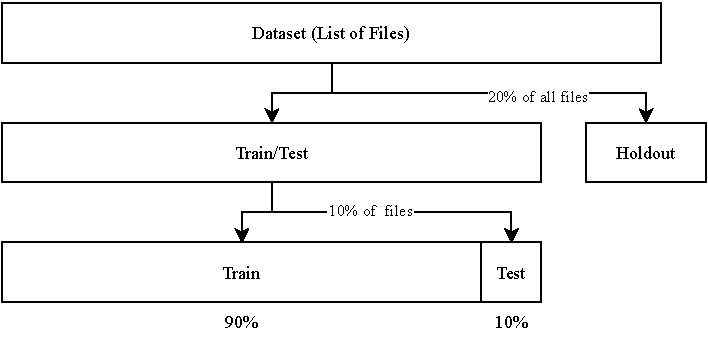
\includegraphics[width=1\textwidth]{img/ML/Data_split.pdf}
    \caption{Split of the dataset. First, 20\% of all files are seperated into a holdout set for later testing. The remainding 80\% of the files are split into 90\% training and 10\% test data. }
    \label{fig:data_split}
\end{figure}

\subsection{Processing}
For the processing steps, we create a pipeline with the d6tflow framework\footnote{\url{https://github.com/d6t/d6tflow}}. Each processing step is a task, that stores its results depending on the parameter configuration in a pickle file. This allows to define a pipeline once and run it with different parameter combinations. The scheduler automatically determines what tasks to run and what task outputs are already stored in pickle files. Consequently, running the pipeline is more efficient and repeatable.

The processing pipeline consists of tasks to read the files into a datastructure, to processes source code and find the problems, to create a vocab dictionary, to convert the data into labeled samples and to split the data into a train, traintest and test set. See \Cref{fig:pipeline_rq2} for a schematic representation of the pipeline.

\begin{figure}
    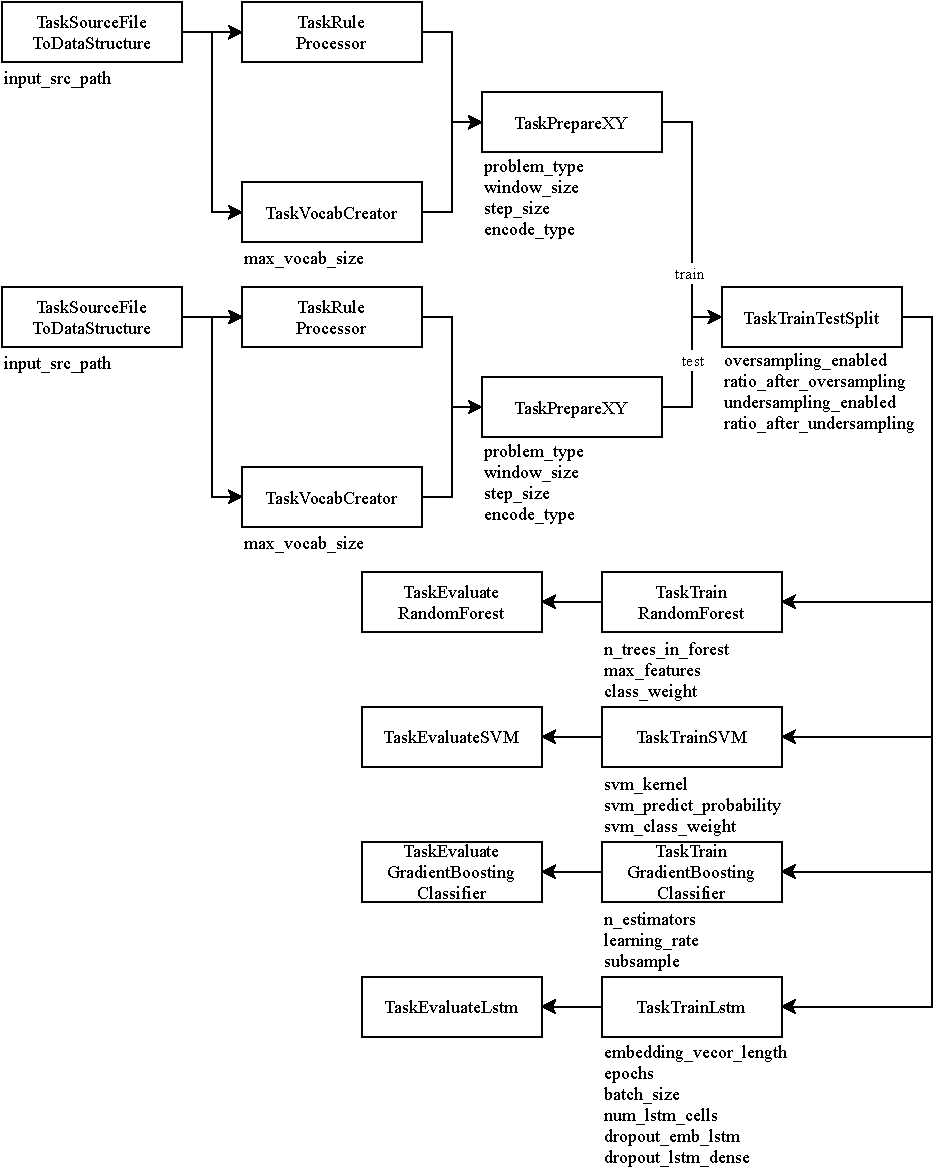
\includegraphics[width=1\textwidth]{img/ML/Pipeline_RQ2.pdf}
    \caption[Schematic representation of the pipeline to train and test models.]{Schematic representation of the pipeline for \hyperref[rq:2]{RQ2} to train and test models with configurable parameters. First, the pipeline reads the source code into memory, extract the vocabulary (\textit{TaskVocabCreator}) and identify all problem types (\textit{TaskRuleProcessor}). It the converts the code of dynamic length into fixed-size samples (\textit{TaskPrepareXY}). This sub-pipeline runs seperate for the train and test set. In \textit{TaskTrainTestSplit}, both datasets are combined and over- or undersampling is applied to the train set. The train set is used to train different classifiers wheras the train and test set are used for evaluation.}
    \label{fig:pipeline_rq2}
\end{figure}


\subsubsection{Files into internal Data Structure}
First, a scanner walks recursively in all subdirectories of the input folder to find all files. If the file has a \textit{.py} extension, its file path and the file content will be stored in a dictionary. The dictionaries for all file are collected into a list. 
Reading all files into main memory increases the performance for downstream tasks, since main memory access is faster than disk access. Although the size of the systems main memory limits the dataset size, a file contains text and is therefore several kilobytes in size. The train dataset with 13,330 files is 86.47MB in accumulated file size.

\subsubsection{Problem Detection}\label{sec:problem_detection}
As a next step, the analysis plugins from the CCAP (see \Cref{sec:analysis_plugins}) process every file and store the line number along with the problem type. As a result, for every file list of problematic line numbers and the corresponding type is available for further processing. The CCAP only covers the two analysis plugins for the problem types CONDITION COMPARISON and RETURN NONE. For model training, we introduce the simple alogrithm to detect comparisons in conditions as problem type CONDITION COMPARISON SIMPLE (described in \Cref{sec:condition_comparison})



\subsubsection{Data Encoding}\label{sec:data_encoding}
The data encoding step transform the internal data representation into input vectors $x$ and output vectors $y$. The transformation is described in the following, multi-stage process.

\paragraph{Fixed Length Sequence}
The length of source code is dynamic, wheras the input size of our models is fixed. Therefore, the character stream of varaible length has to be transformed into a token stream of fixed size. 
To extract meaningful tokens from the character stream, we use the python tokenizer from its standard library. The tokenizer seperates the character stream based on the python syntax definition into tokens. All tokens contain a token type (like a name or operator token), the corresponding characters in the source code and a start and end position (line and column number). Next, the token stream is divided into a fixed size token sequence using a sliding window aproach (size: 20, step size: 3).
\paragraph{Vocabulary Creation}
To represent a token value with a number, every token value needs a numeric representation. Therefore, the occurence of each token value is counted and the index in an descending ordered list for each token value represents the token as an integer. To ignore potential capitalization missmatches, all token values are lower-case. The overall size of the vocabulary is configurable. If the size is smaller than the size of the distinct token value set, the least common token values will be replaced by an unknown token. The unknown token has a numeric representation one bigger than the vocabulary size. We found that using a vocabulary size of 100,000 results in an acceptable 3.9\% unknown token frequency.
\paragraph{Index-Based Encoding}
The textual token values are encoded with an Index-Based encoding. The most common token values have a numerical representation based on their index in a vocabulary (created with all token values of the train data). Optional, the type of each token is encoded by its numerical representation in the standard library. The type and value encoding are then combined alternating in a final encoding vector that represents an input sample.
\paragraph{Label Extraction}
With the internal representation, the ground truth is encoded as a line number. A transformation is necessary to label each sample corresponding to a given problem type. Label 1 is assigned, if the sample contains the given problem type. A sample contains a problem type, if it contains all tokens from the problematic line. If the sample is missing a token of the problematic line at the beginning or end, the label is 0 for non-problematic code. 

\subsubsection{Train/Test Split}\label{sec:train_test_split}
In \Cref{chap:clean_code_classification_dataset}, we described to create a train, test and holdout dataset by file level seperation and not by sample level splitting.
Since we use a sliding window approach to convert source files with dynamic length into fixed length token sample samples, we may have one problematic code line in multple samples. If we would do a train/test split on sample level, we may indroduce samples covering one problematic pattern at different positions in both datasets. \Cref{fig:encoding_sliding_window} illustrates multiple windows covering one sample. This unclean separation would diminish the validity of metrics calculated from the test and holdout dataset. 
\begin{figure}
    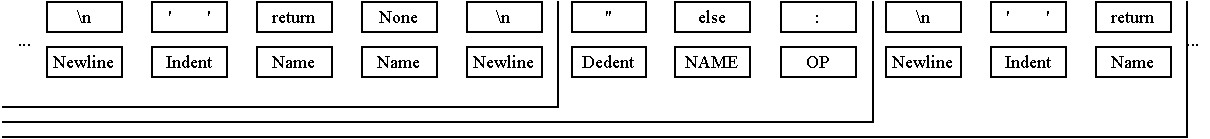
\includegraphics[width=1\textwidth]{img/ML/encoding_sliding_window_problem.pdf}
    \caption[Sliding window approach on source code containing a problematic \texttt{return None}]{Sliding window approach on source code containing a problematic \texttt{return None}. Multiple windows will contain the problematic sample. Consequently, we can not split on sample level, since the same problem would be in the train and test set. Instead, we split on file level to have a clean separtion between the datasets.}
    \label{fig:encoding_sliding_window}
\end{figure}

\subsubsection{Code Manipulation}\label{sec:approach_code_manipulation}
In research question \hyperref[rq:3]{RQ3}, we evaluate the models generalisation to detect similar pattern the model was not trained on. Therefore, we manipulate the code that it is still a rule violation, but the original analysis plugins would not spot them. The pipeline for code manipulation differ from the pipeline for RQ2 by an additional code manipulation task and a removal of the training step (see \Cref{fig:pipeline_RQ3}).

\begin{figure}
    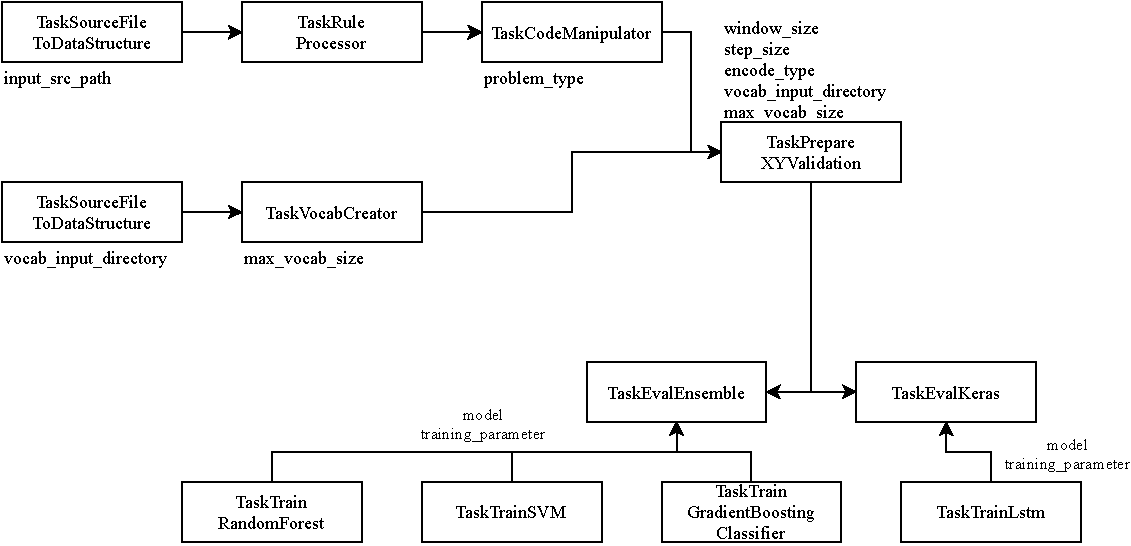
\includegraphics[width=1\textwidth]{img/ML/Pipeline_RQ3.pdf}
    \caption[Pipeline for code manipulation and evaluation.]{Pipeline for code manipulation and evaluation. The prerpocessing part is like in \Cref{fig:pipeline_rq2} but with an additional \textit{TaskCodeManipulator} to manipulate the code as described in \Cref{sec:approach_code_manipulation}. The random forest classifier, svm and gradient boosting classifier require different evaluation code as the LSTM, so two \textit{TaskEval*} are used. }
    \label{fig:pipeline_RQ3}
\end{figure}


\paragraph{Return None}\label{par:manipulation_return_none}
For the problem type RETURN NONE, we manipulate the code to have an inline if statement that only returns None in one branch. Therefore, a function may still return None, but the analysis plugin would not detect this. \Cref{lst:return_none_modified} shows an example for this case. Although a modification of the analysis plugin could cover the variations as well, we want to see how well machine learning models could perform on this task.

To modify the original code, we use the preprocessed code with problems detected as in \Cref{sec:problem_detection}. For every source code line containing the RETURN NONE problem, we use regular expressions to replace the \textit{return None} with a variation as seen in \Cref{lst:return_none_modified}. 

The following data encoding step is similiar to the one for model training, although this modified samples will only be used during evaluation.

\begin{minipage}[c]{\linewidth}
\begin{lstlisting}[language=Python, label=lst:return_none_modified, caption={Samples for returning None. The first return would be flagged by the analysis plugin, the second and third return are modified variations that would be ignored by the analysis plugin. The performance of the machine learning models on detecting the latter will be evaluated.}]
def f(a,b):
    #detected by the analysis plugin
    return None 

    #not detected by the analysis plugin
    return None if a < b else b 

    #not detected by the analysis plugin
    return a if a < b else None \end{lstlisting}
\end{minipage}
\paragraph{Condition Comparison}
The analysis for the CONDITION COMPARISON problem type is an advancement of the analysis of the CONDITION COMPARISON SIMPLE problem type.  See \Cref{lst:conidtion_comparison_modified} for examples of the different analysis results.
Since the results of CONDITION COMPARISON are the modification of the CONDITION COMPARISON SIMPLE, we use the first as ground truth for evaluating the generalisation. Since the CONDITION COMPARISON SIMPLE problems are a subset of the CONDITION COMPARISON problems, we use a similar approach as before (see \Cref{par:manipulation_return_none}) to transform all problem occurances to be undectable by the CONDITION COMPARISON SIMPLE analysis plugin.

\begin{lstlisting}[language=Python, label=lst:conidtion_comparison_modified, caption={Sample statements for the differnce between the two analysis plugins CONDITION COMPARISON and CONDITION COMPARISON SIMPLE.  }]
    def f(a,b):
    #detected by CONDITION COMPARISON SIMPLE
    #detected by CONDITION COMPARISON
    if a < b:
        pass 

    #not detected by CONDITION COMPARISON SIMPLE
    #detected by CONDITION COMPARISON
    if not a < b:
        pass 

    #not detected by CONDITION COMPARISON SIMPLE
    #detected by CONDITION COMPARISON
    if isSmaller(a,b) or a < b:
        pass \end{lstlisting}

\subsection{Models}
Classifying code samples is a binary classification problem since we consider each problem type as a seperate classification task. We train and evaluate a random forest classifier, a support-vector machine based classifier, a gradient boosting classifier and a neural network with LSTM cells.

\paragraph{Random Forest}
We use a random forest classifier with 100 decision trees to perform the binary classification. Additional to over- and undersampling, we experiment with an automatic class weighting inverse proportional to class frequency. The other hyperparamter follow the default implementation of the scikit-learn library: The quality measure of a split follows the gini function, the tree depth is unlimited and the number of features to consider for each split is the square-root of the number of features overall.
\paragraph{Support Vector Machine}
We use the support vector classification from the scikit-learn library. As a kernel function, we choose the radial basis function for a performance baseline. Additionally, we try the class weighting inverse proportional to the class frequency to combat the inbalanced dataset.
\paragraph{Gradient Boosting Classifier}
For gradient boosting classifier, we mainly vary the number of boosting steps and the learning rate. Furthermore, we experiment with stochastic gradient boosting by setting the subsample parameter to 0.4 and 0.7. Other hyperparameter settings follow the default value of the scikit-learn library.
\paragraph{Neural Networks with LSTM Cells}
Our neural network consists of five layer (see \Cref{lst:lstm}). First, we use an embedding layer with an embedding size of 32. The input is the Index-Based encoded samples without type encoding. This layer is trained end-to-end with the complete network on the trainings-data. Furthermore, this layer covers most trainable parameters of the model. As a hidden layer, we use 10 LSTM cells with a prior and posterior dropout layer with a default 0.2 dropout. To perform binary classification, our model ends with a dense mapping onto a single neuron. The binary result is determined based on a 0.5 threshold for the output of the last neuron.

We vary the hyperparameters for batch size, number of epochs, embedding size and number of LSTM cells.

\begin{lstlisting}[label=lst:lstm, caption={Summary of our LSTM network. We use an embedding layer of size 32, 10 LSTM cells, a dropout layer before and after the LSTM layer with a defaut dropout ratio of 0.2 and a dense mapping to a single output neuron for binary classifcation with a threshold of 0.5.}]
Layer (type)                 Output Shape              Param #
============================================
embedding (Embedding)        (None, 20, 32)            3200064
__________________________
dropout (Dropout)            (None, 20, 32)            0
__________________________
lstm (LSTM)                  (None, 10)                1720
__________________________
dropout_1 (Dropout)          (None, 10)                0
__________________________
dense (Dense)                (None, 1)                 11
============================================
Total params: 3,201,795
Trainable params: 3,201,795
Non-trainable params: 0\end{lstlisting}

\chapter{Quantitative Evaluation}
Research questions
Description of the evaluation environment/setup
Results/answers per research question
Optional comparison to prior work
Discussion and analysis of strengths/problems
Note: see 

\section{Research Questions}

\begin{description}
    \item[RQ1] Can the Clean Code Analysis Platform be a useful addition to developers workflow besides existing tools? 
    \item[RQ2] What models perform well on detecting non-clean code
\end{description}

\subsection{RQ1: Can the Clean Code Analysis Platform be a useful addition to developers workflow besides existing tools?}
\paragraph{Motivation}
Several tools are established that aim to improve code quality and detect unclean code. Every new tool with similar claims has to prove its usefulness beside the preexisting tools. We compare the CCAP with existing tools based on the design goals expandability, useability and integration. Additionally, we will mention and compare useful features unique to existing tools.
\paragraph{Approach}
To evaluate, if the CCAP is a useful addition, we compare different features to see, if it can supplement or replace existing tools. As described in section TODO, the compared tools are Sonarcube, PMD Source Code Analyser Project, Codacy and PyLint.

\paragraph{Results}
Table TODO shows a summary of the features.

\subparagraph{Finding 1: Expandability}
For expandability of analysis plugins, CCAP is comparable to PyLint, that also offer plugins to analyse the raw string, the token stream or the AST. PMD allows plugins to analyse the AST or define XPath rules. Since XPath rules can be used in the CCAP as well (using a third-party library in the plugin), PMD offers fewer expansion possibilities. Sonarqube, on the other hand, provides the most possibilities for extension. Not only can developers analyse the AST, specify XPath rules, but they have access to an additional semantic model of the code that provides direct access to structures such as methods, parameters, return values. This semantic model simplifies analysis in comparison to the AST analysis.
Additionally, Sonarqube allows plugins to expose an API for other plugins to use. This different type of plugin further increases the possibilities for rule checking plugins. The least expandability offers Codacy, that allow customising or disabling existing rules, but does not offer to add rules to the existing ruleset.

Regarding output plugins, no compared tool offers the output customisation of CCAP. PMD and PyLint have different predefined output formats like JSON, HTML, CSV or text. Although PyLint allows customising the message format using a formatting string as a command-line argument, they do not offer extensions for the output. Sonarqube displays the analysis reports in its WebUI. The scanner tool, SonarScanner, sends the reports to the server component, that renders the results in the browser.  Codacy's local scanner produces text output; the cloud version also has a WebUI.

\subparagraph{Finding 2: Integration shortcomings}
The CCAP has significant shortcomings in its integrations into IDEs, build processes and CI pipelines. All contestant tools provide plugins for build systems like Gradle or Maven. Except for Codacy, all tools have IDE integrations into the most common editors. Sonarqube and Codacy have integrations into source control systems. Same applies to PMD and PyLint since they are included in Codacy and therefore have the same integrations.

\subparagraph{Finding 3: Useability}
For a plugin developer, the useability of the plugin system is simple for CCAP and PyLint. Both tools have the same plugin mechanism and a simple plugin interface to work with. PMD has a similar, straightforward plugin interface, but its Java plugin has to be bundled into a jar file before adding to the classpath. The latter applies to Sonarqube as well; additionally, the powerful and rich plugin API makes it harder to use.

For the user, installing CCAP is like installing every other python package. Running from the command-line is fast and can be automated, e.g. using git pre-commit hooks. The same workflow would be achieved with PyLint. Sonarqube is more complex to install due to its multiple components, but after the setup, the WebUI and integrations into most developer workflow have the best useability. Codacy as a cloud service only requires permission to access the source code repository to start scanning the code.

\subparagraph{Finding 4: Multi-Language scanning}
Sonarqube, PMD and Codacy offer multi-language scanning. This multi-language ability is advantageous for code repositories with multiple languages and for reusing the same tools and infrastructure for multiple projects with different programming languages. Supporting multi-language scanning is not possible with CCAP and would require a redefinition of the architecture. Although multi-language support was not a design goal, it would be a significant advantage for adoption.

\subparagraph{Finding 5: Maturity and Community-Support}
The maturity and community-support of tools impact the integration of the tools into the developer workflow. Some integrations are community-made and shared, so everybody has an advantage. The community support would also be necessary for CCAP to write and share additional analysis plugins and to integrate into different workflows.

\paragraph{Summary}
In summary, CCAP offers a good, but not best in class expandability with analysis plugins. It has a high useability for plugin developer and users. The lack of integrations for different workflows reflects the lack of community support and maturity. 
We see the CCAP as an addition to the powerful Sonarqube. The simple, yet robust expandability of the CCAP could supplement the shortcomings of Sonarqube in its powerful, but complex expandability. For instance, a code reviewer could code problematic code into a simple python plugin, distributes it to the team and would hopefully not reencounter the same problem.
Additionally, the CCAP could be used to teach about Clean Code and to enforce specific coding rules to students, since the local setup is straightforward. Clean Code rules could be turned into analysis plugins by students or teachers without having to understand a complicated interface.

\subsection{RQ2: What models perform well on detecting non-clean code?}
\paragraph{Motivation}
As we have shown with the CCAP and the analysis plugins, it is possible to write an algorithm that can detect certain code patterns like non-clean code patterns. If we are able to write a well tested detection algorithm, we do not need error-prone machine learning models to detect code patterns. Nonetheless, if we can not design an algorithm that detect a desired code pattern reliablely, we may perform better using a machine learning model. Additionally, if we encode a subjective pattern, it may not be possible to design an algorithm to objectively detect such a pattern. As a solution, we could label code parts as our pattern and use machine learning approches to implicitly extract rules to detect such a pattern.

For this research question, we will evaluate different machine learning models on different code patterns and compare the results.

\paragraph{Approach}
For answering the research question, we will use the approach detailed in chapter \ref{chap:clean_code_classification}.  The dataset, consisting of 18 projects from GitHub, is prepared as described in chapter \ref{chap:clean_code_classification_dataset}. The data is split into 90\% train and 10\% test data. We use the train dataset to train Random Forest, Gradient Boosting Classifier, Support Vector Machines and a LSTM-based neural network. Due to the class inbalance, we will additional train with an oversampled dataset (oversampling rate of 0.5) and an undersampled dataset (undersampling rate of 0.5). Since our test set contains real-world code samples, we expect it to reperesent a real-world label distribution and we therefore accept potential effects of the data inbalance. Nevertheless, we will try to train with an over- and undersampled dataset to observe the effect on the performance.

Our evaluation metrics are recall, precision and the combined f1 score. Due to the data inbalance, accuracy is not a meaningful metric. A high recall means a high detection rate of non-clean code. The cost of a false negative prediction are potential costs in unclean code (maintainability, understandability). With a high precision, a detected non-clean code sample is likely to be a non-clean code sample and the system reports less false positives. The immediate cost of false positive predictions (resulting in a lower precision) are the extra developer time needed. Additionally, the cry wolf effect (TODO source) comes into play. In our case, a developer who has seen a false alarm will take subsequent alarms less serious. Additionally, a study has shown that a higher false alarm rate in advisory warning system in cars results in a lower, subjective evaluation of the system (TODO source Cooperative warning systems: The impact of false and unnecessary alarms on drivers’ compliance). A low subjective evaluation of developers would lead to a decrease in adoption rate which consequently lead to more unfixed problematic code. Since both, recall and precision are important to the success of our models, we decided to use the equally weighted f1 score as single-value evaluation metric.
Additionally, to compensate the cascading effect of a low precision, we require a precision of 0.8 as a satisficing metric. This means, we accept all models that return two false positive and eight true positive samples. On the other hand, we define the recall as our optimizing metric.

We evaluate all models for the three different problem types RETURN\_NONE, CONDITION\_COMPARISON\_SIMPLE and CONDITION\_COMPARISON.

\paragraph{Results}
Table TODO shows the best performing hyperparameter per model for all three problem types. Figure TODO shows the confusion matrix those model configurations. We list all hyperparameter configurations and the corresponding traing, train/test and test pefromance for all problem types in the appendix (Table \ref{tab:all_results_random_forest}-\ref{tab:all_results_svm}).


% Please add the following required packages to your document preamble:
% \usepackage{booktabs}
\begin{table}[]
    \begin{tabularx}{\textwidth}{rXXX}
    \toprule
    \multicolumn{1}{l}{}                             & RN         & CCS & CC \\ \midrule
    \multicolumn{1}{l}{Random Forest}                & \multicolumn{1}{r}{} &            &              \\
    F1                                               & 0.8486               & 0.9352     & 0.9351       \\
    Recall                                           & 0.7404               & 0.8936     & 0.8976       \\
    Precision                                        & 0.9939               & 0.9809     & 0.9759       \\ \midrule
    \multicolumn{1}{l}{SVM}                          &                      &            &              \\
    F1                                               &   0.0066             &  0.0622    &   0.1115     \\
    Recall                                           &   0.0134             &  0.5004    &   0.5535     \\
    Precision                                        &   0.0044             &  0.0332    &   0.062      \\ \midrule
    \multicolumn{1}{l}{Gradient Boosting Classifier} &                      &            &              \\
    F1                                               & 0.9328               & 0.8489     & 0.9088       \\
    Recall                                           & 0.9005               & 0.7953     & 0.8766       \\
    Precision                                        & 0.9675               & 0.9102     & 0.9434       \\ \midrule
    \multicolumn{1}{l}{LSTM}                         &                      &            &              \\
    F1                                               & 0.9933               & 0.9805     & 0.9783       \\
    Recall                                           & 0.9933               & 0.9779     & 0.9868       \\
    Precision                                        & 0.9933               & 0.9831     & 0.97       \\ \bottomrule
    \end{tabularx}
    \caption{Best performing classifier for RQ2 based on f1 score of the holdout set. For the SVM, the validation performance of the configuration with available data is used.}
    \label{tab:rq2_best_classifier}
    \end{table}

\subparagraph{Finding 1: poor SVM performance}
SVM performed poorly. Based on the f1 score, the best configuration has a f1 of 0.0066, a recall of 0.0134 and a precision of 0.0044. In other words, only 1.34\% of positive samples are recognized as positive. The model seems to fail to seperate the two classes. A reason may be the class inbalance, since only 0.21\% of all samples of are non-clean code (positive) with the RETURN\_NONE type. In this configuration, we used undersampling with a ratio of 0.5, since oversampling was not feasable due to the increase in train time (see section \ref{sec:svm_quadratic_complexity}). After undersampling, 1/3 of all samples are therefore positive and 2/3 are negative. Since the time to train is still too long, we only took half of the undersampled dataset. 

We additionally used the svm in a configuration with an automatic class weigthing that is inverse-proportional to the class frequency. The recall score increases by 57-fold to 0.7660 wheras the precision decrease by half to 0.0026. We conclude, that the svm is very sensitive to class inbalance, which is an improper characteristic for our inbalanced classification problem. Additionally, a precision of 0.0026 is not useable for any application. We can not boost the precision with more data to help the model to distinguish true positives and false positives, since the train time will increase quadratically. We a baseline that low we do not expect much improvement with further investigation and therefore conclude that there is no valid reason to further invest in the svm model.


\subparagraph{Finding 2: Random Forest}
Generally, the random forest classifier performs with a f1 score over 0.8 over all problem types with an oversampling ratio of 0.5, 100 trees, no additional class weighting and type encoding. For RN, this configuration has a 0.8379 f1, 0.7221 recall and 0.9978 precision on the test dataset. For CCS and CC, the f1 with 0.9329 and 0.929 are even better. The recall for those problem types increases to 0.8898 and 0.8888 while the precision remains high with 0.9803 and 0.9731 respectively. The random forest clasifier therefore fullfills our satisficing condition of a precision higher than 0.8.

Generally, we obeserve a performance increase by applying oversampling, especially for the RN problem type. From an f1 score of 0.7699 for 100 trees, no additional class balance and type encoding to 0.8379 with an oversampling ration of 0.5. Since only TODO \% of RN train samples are positive, oversampling those to half of the number of majority samples will lead to a bigger increase in training samples than oversampling less inbalanced problem types such as CCS and CC. This explains the better performance of the latter problem types, since the oversampled train dataset is larger than for RN. Furthermore, we observe a neglegtable difference of 0.02 in f1 score for oversampling to a ration of 1.0 (same amount of samples for both labels).

Another common pattern is a worse performance on undersampled train sets. We observe a significant drop in performance for the RN problem type, if we use a 0.5 undersampling ratio. Similiarly, the performance for CCS and CC drops, although the decrease is smaller. Furthermore, we observe a moderate performance drop with 0.1 undersampling. From this pattern and the afforementioned oberservations for oversampling, we infer that a random forest classifier can profit from more data, even if they contain duplicated samples for the minority class due to oversampling. This can also explain the larger drop for undersampling for the RN problem type, since the non-clean code class contains less samples for RN than for CCS and CC (TODO numders of samples in train dataset). With less samples, the undersampling process reduces the overall amount of samples by deleting samples from the majority class. With an undersampling ratio of 0.1, less examples are deleted and the effect is less impactful, but still observable. This effect is also visible in the smaller difference in performance between the CCs and CC problem type with undersampling. For CCS, the random forest classifier performs slightly worse than for CC, since only TODO samples have a CCS problem type whereas TODO samples contain the CC problem type.

The impact of class weighting in comparison to equivalent configurations seems to be neglegtable. 
mention numbers to proove the point
To evaluate the impact of class weighting, we compare the variation in this parameter with otherwise identical configurations.
For an oversampling ratio of 0.5 with type encoding, we see 0.8379, 0.9329 and 0.929 in test f1 perfromance without class weigthing and 0.8352(-0.0027), 0.9287(-0.0042) and 0.9267(-0.0023) in test f1 score performance. The difference is not significant.
For undersampling with a ratio of 0.5 and type encoding, the f1 score changes from 0.2583, 0.806 and 0.8632 test f1 score without class weighting to 0.2709(+0.0126), 0.8111(+0.0051) and 0.8671(+0.0039) test f1 score with class weighting. Again, the difference is not significant.
Without resampling and without type encoding, the f1 test performance decreases from 0.7814, 0.9057 and 0.9116 without class weighting to 0.7475(-0.0339), 0.8894(-0.0163) and 0.8913(-0.0203) with class weighting.
Last, without resampling but with type encoding, the f1 test score decreases from 0.7699, 0.9208 and 0.9211 without class weighting to 0.7506(-0.0193), 0.9064(-0.0144) and 0.9071(-0.014) with class weighting.
All changes due to class weighting are not significant so class weighting does not have any positive influence on the performance of the random forest classifier.

Enabling type encoding improves our f1 performance for all configurations over all problem types except for the RN type without over- or undersampling. We already mentioned the extreme class inbalance for the RN problem type and therefore accept this type as outlier to the general observation. The improvement in f1 scores is due to the improvement in recall of around 0.02 for all problem types excluding the afforementioned exception. This data implies that the additional type information are useful to more reliablely determine our kinds of problematic code. We guess this boils down to the smaller variance in token types. For example, a string token is always treaded as the same token no matter the content. Since the content could change and may not be included in the dictionary, the variance in the type encoding is lower and therefore easier to learn. TODO print feature importance!!!

Overall, it seems like a random forest classifier can handle class inbalance fairly well, as long as distribution is not too unbalanced as for RN problem type. The performance deteriotes if the inbalance superceeds a critical threshold (for RN), otherwise it has minor impact.
We base this conclusion on several observations: First, we see a better performance for the CCS and CC problem type overall, both of which have a more blanced distribution than the RN problem type although. It is important to note, that the different problem types also have different difficulty levels for the model. But we assume the RN type is easier to detect for a model, since the model only has to learn two subsequent tokens anywhere in the sequence. Therefore, we attribute this effect to the class distribution, but we remark that this may be tested in an additional, isolated experiment. Second, without over- or undersampling, we observe similar performance for CCS and CC, despite their different frequency in the train set (TODO: class frequency values). And finally, we would expect a bigger impact of class balancing, if the random forest classifier would be sensitive to class inbalance.
Additionally, encoding the token types results in a better performance than only encoding token values.

overfitting for random forest

\subparagraph{Finding 3: Gradient Boosting Classifier}
The overall best performing gradient boosting works with 300 boosting steps and a learning rate of 0.2. For the RN problem type, it delivers a f1 score of 0.9196, a recall score of 0.8666 and a precision of 0.9796. Compareable performance is measured for the CC type: 0.9008 f1, 0.8673 recall and 0.937 precision. The performance decreases for the CCS type to 0.8419 f1, 0.7902 recall and 0.9009 precision for the same, best performing configuration. A decrease in performance for the CCS problem type applies to all configuration in compraison to the CC type. Nevertheless, the gradient boosting classifier fullfills our satisficing criteria of a precision score higher than 0.8.

Over- and undersampling does not have a positive effect: The f1 score of the 200 stages, 0.2 learning rate and 1.0 subsampling drops by 0.3459 for a 0.5 oversampling ratio for the RN problem type. With an undersampling ratio of 0.5, the f1 score decreases by 0.3761 to 0.4545 on the test set. The performance deteriotion for the CCS and CC type are lower but still significant: For CCS, the f1 score drops by 0.0782 to 0.6948 with oversampling and by 0.0494 to 0.6836 with undersampling. Using over- or undersampling as rebalancing strategies does not improve the classifiers performance. The best classifier configuration performs better on the RN and CC problem type compared to the CCS problem type (0.9196 and 0.9008 vs. 0.84119 f1 on test dataset). This allows two implications: Since the RN type is strongly underrepresented in the train set (class frequency of TODO) compared to the CCS class (TODO class frequency), the gradient boosting classifier does not suffer from strong class inbalances. On the other hand, the CCS problem type seems harder to learn, contradictory to our assumptions about the difficulty levels of the different problem types.

Furthermore, we we experimented with giving only a subsample of the train data to the individial base learners for fitting (subsampling ratio of 0.7 and 0.4). Since we see the exact same performance metrics, this hyperparameter has no effect on the models performance.

By contrast, increasing the number boosting stages improves every precision metric for all problem types. From a f1 score of 0.6177, 0.5974 and 0.7314 for RN, CCS and CC at 100 boosting stages, we observe a improvement to 0.8306, 0.774 and 0.8567 at 200 boosting stages and 0.9196, 0.8419 and 0.9008 at 300 boosting stages. Additionally, the train performance for these configuration is similiar to the the test and holdout performance. Consequently the classifier does not overfit on the train data and we could further increase the boosting stages to further improve the performance. Since additional boosting stages increase the train time of the model, we did not investigated further into this direction, but we expect by increasing the boosting stages and tuning the learn rate correspondingly, one could maximize the perofrmance. 

In conclusion, the gradient boosting classifier is robust to overfitting and rather improves its performance with more boosting steps. We could also observe a robustnes for class inbalance and we therefore do not profit from our over- and undersampling approach. Subsampling has no effect and we observe an unexpected high difficulty of learning the CCS type for this classifier.




TODO: write in approach what we vary
- classify the problems into difeent difficulties

\chapter{Conclusion}
An overall short summary of results
What was successful, what not (and hypotheses why)
Hints for further future work/extension

\section{Summary}
Software maintenance is a considerable cost factor for software development. With high code quality, the maintenance efforts can be optimised. With the clean code principles, developers have a ruleset to write understandable and readable code that will positively impact code quality. The focus of this thesis lies on the automated checking of such rules.

We introduced a taxonomy of complexity level for the clean code rules, depending on the level of complexity for an automated checker. On the highest level, we grouped clean code rules that would potentially require machine-learning approaches to learn the detection of a rule violation. 

The contribution of this work is twofold: 
First, we designed an implemented the clean code analysis platform (CCAP). It is a tool that checks for clean code violations. One of the essential design aspects is the easiness to extend the tool to cover additional clean code rules. In comparison with preexisting tools, we see a high value for users and extension developers, that write automated checker for new rules. On the downside, it lacks the integration into different workflows. The CCAP is an addition to Sonarqube. The strength in extensibility supplement the rather complicated extensibility of Sonarqube. Furthermore, CCAP is a useful tool to teach about clean code principles.

Second, we compared different machine learning models on detecting violating code pattern. A support vector classifier was not able to complete the task with acceptable performance. The LSTM-based neural network outperforms all other models on the task, but it is sensitive towards less training data due to many trainable parameters.
A random forest classifier fulfiled our acceptance criteria. It can handle moderate class imbalance and profit from oversampling the training samples. The gradient boosting classifier is insensitive towards class imbalance which is a useful property for the task. When classifying for a single clean code violation, most lines of code do not contain the violating pattern, so the training dataset is imbalanced. The gradient boosting classifier also fulfils our acceptance criteria and performs better than the random forest on two out of three problematic code patterns.

Furthermore, we tried to simulate a situation in which the dataset may not cover the full variety of possible problem patterns. We tested the trained models on unseen problem variations. No model performed on an acceptable level. We assume, our models did not learn the structure of the problematic pattern but just the possible variations. 
We think of two main reasons: First, the variation in the training set is too limited for the model to extract the general structure. We suggest to explicitly introduce variety by hand-generating different patterns to fine-tune the model and to use in the test set for hyperparameter tuning.
Second, our encoding approach does not utilise the structure of the source code. Since our models did not extract the structure from our encoding, encoding the structure as input features would ease the learning of the problem structure.  

\section{Future Work}
TODO

  

\clearpage

\bibliographystyle{plain}
\bibliography{references}

\appendix
\appendixpage
\addappheadtotoc
\setcounter{table}{0}
\renewcommand{\thetable}{A\arabic{table}}

\chapter{RQ2: Model Performances}
\begin{table}[]
    \tiny
    \tabcolsep=0.11cm
    \begin{tabularx}{\textwidth}{XXXXX|X|XXX|XXX|XXX}
    \toprule
    \multicolumn{5}{c}{Parameter} & \multicolumn{3}{c}{RN} & \multicolumn{3}{c}{CCS} & \multicolumn{3}{c}{CC} \\ \midrule
    over-\newline samp. & under-\newline samp. & \#trees & class\newline weight & encode\newline type  & & Train &  Test & Holdout & Train &  Test & Holdout & Train &  Test & Holdout \\ \midrule
    0.5 & - & 100.0 & None & True& & & & & & & & & \\
    & & & & & \textit{F1} & 1.0 & 0.8379 & 0.8486 & 1.0 & 0.9329        & 0.9352        & 1.0        & 0.929        & 0.9351        \\
    & & & & & \textit{Rec} & 1.0 & 0.7221 & 0.7404    & 1.0 & 0.8898    & 0.8936    & 1.0    & 0.8888    & 0.8976    \\
    & & & & & \textit{Prec} & 1.0 & 0.9978 & 0.9939 & 1.0 & 0.9803 & 0.9809 & 1.0 & 0.9731 & 0.9759 \\ \midrule
    1.0 & - & 100.0 & None & True& & & & & & & & & \\
    & & & & & \textit{F1} & 1.0 & 0.8358 & 0.8367 & 1.0 & 0.9287        & 0.9322        & 1.0        & 0.9273        & 0.9324        \\
    & & & & & \textit{Rec} & 1.0 & 0.719 & 0.7225    & 1.0 & 0.8824    & 0.8876    & 1.0    & 0.8853    & 0.8925    \\
    & & & & & \textit{Prec} & 1.0 & 0.9978 & 0.9937 & 1.0 & 0.9801 & 0.9815 & 1.0 & 0.9736 & 0.9761 \\ \midrule
    0.5 & - & 100.0 & balanced & True& & & & & & & & & \\
    & & & & & \textit{F1} & 1.0 & 0.8352 & 0.8385 & 1.0 & 0.9287        & 0.9321        & 1.0        & 0.9267        & 0.9329        \\
    & & & & & \textit{Rec} & 1.0 & 0.7182 & 0.7249    & 1.0 & 0.8826    & 0.8882    & 1.0    & 0.885    & 0.893    \\
    & & & & & \textit{Prec} & 1.0 & 0.9978 & 0.9942 & 1.0 & 0.9799 & 0.9806 & 1.0 & 0.9727 & 0.9765 \\ \midrule
    0.5 & - & 100.0 & None & False& & & & & & & & & \\
    & & & & & \textit{F1} & 1.0 & 0.8287 & 0.8519 & 1.0 & 0.9191        & 0.9217        & 1.0        & 0.921        & 0.9248        \\
    & & & & & \textit{Rec} & 1.0 & 0.708 & 0.7453    & 1.0 & 0.869    & 0.8723    & 1.0    & 0.8736    & 0.8785    \\
    & & & & & \textit{Prec} & 1.0 & 0.9989 & 0.9939 & 1.0 & 0.9752 & 0.977 & 1.0 & 0.9739 & 0.9764 \\ \midrule
    1.0 & - & 100.0 & None & False& & & & & & & & & \\
    & & & & & \textit{F1} & 1.0 & 0.8162 & 0.8268 & 1.0 & 0.9189        & 0.9186        & 1.0        & 0.9161        & 0.9214        \\
    & & & & & \textit{Rec} & 1.0 & 0.69 & 0.7084    & 1.0 & 0.8692    & 0.8674    & 1.0    & 0.8656    & 0.872    \\
    & & & & & \textit{Prec} & 1.0 & 0.9989 & 0.9926 & 1.0 & 0.9747 & 0.9763 & 1.0 & 0.9729 & 0.9767 \\ \midrule
    - & - & 100.0 & None & False& & & & & & & & & \\
    & & & & & \textit{F1} & 0.9999 & 0.7814 & 0.7987 & 0.9998 & 0.9057        & 0.9106        & 0.9998        & 0.9116        & 0.9173        \\
    & & & & & \textit{Rec} & 0.9998 & 0.6413 & 0.6658    & 0.9999 & 0.8406    & 0.8489    & 0.9998    & 0.8495    & 0.8571    \\
    & & & & & \textit{Prec} & 1.0 & 1.0 & 0.9979 & 0.9998 & 0.9818 & 0.982 & 0.9998 & 0.9835 & 0.9866 \\ \midrule
    - & - & 100.0 & None & True& & & & & & & & & \\
    & & & & & \textit{F1} & 0.9999 & 0.7699 & 0.7666 & 0.9998 & 0.9208        & 0.9243        & 0.9998        & 0.9211        & 0.9269        \\
    & & & & & \textit{Rec} & 0.9998 & 0.6264 & 0.6226    & 0.9999 & 0.8637    & 0.8694    & 0.9998    & 0.8675    & 0.8759    \\
    & & & & & \textit{Prec} & 1.0 & 0.9987 & 0.9972 & 0.9998 & 0.9859 & 0.9865 & 0.9998 & 0.9817 & 0.9841 \\ \midrule
    - & - & 100.0 & balanced & True& & & & & & & & & \\
    & & & & & \textit{F1} & 0.9999 & 0.7506 & 0.7503 & 0.9998 & 0.9064        & 0.9087        & 0.9998        & 0.9071        & 0.9121        \\
    & & & & & \textit{Rec} & 1.0 & 0.6013 & 0.6018    & 1.0 & 0.8385    & 0.8404    & 1.0    & 0.8414    & 0.8484    \\
    & & & & & \textit{Prec} & 0.9997 & 0.9987 & 0.9959 & 0.9996 & 0.9863 & 0.9891 & 0.9997 & 0.9839 & 0.9863 \\ \midrule
    - & - & 100.0 & balanced & False& & & & & & & & & \\
    & & & & & \textit{F1} & 0.9999 & 0.7475 & 0.7405 & 0.9998 & 0.8894        & 0.8924        & 0.9998        & 0.8913        & 0.898        \\
    & & & & & \textit{Rec} & 1.0 & 0.5973 & 0.5888    & 1.0 & 0.8112    & 0.8149    & 1.0    & 0.8136    & 0.8227    \\
    & & & & & \textit{Prec} & 0.9997 & 0.9987 & 0.9976 & 0.9996 & 0.9843 & 0.9863 & 0.9997 & 0.9853 & 0.9885 \\ \midrule
    - & 0.1 & 100.0 & None & True& & & & & & & & & \\
    & & & & & \textit{F1} & 1.0 & 0.6857 & 0.654 & 0.9999 & 0.9268        & 0.928        & 0.9999        & 0.929        & 0.9345        \\
    & & & & & \textit{Rec} & 1.0 & 0.9027 & 0.9275    & 1.0 & 0.92    & 0.9243    & 0.9999    & 0.8981    & 0.9064    \\
    & & & & & \textit{Prec} & 1.0 & 0.5529 & 0.5051 & 0.9999 & 0.9336 & 0.9317 & 0.9999 & 0.9621 & 0.9644 \\ \midrule
    - & 0.5 & 100.0 & None & False& & & & & & & & & \\
    & & & & & \textit{F1} & 1.0 & 0.3469 & 0.3024 & 1.0 & 0.8087        & 0.8157        & 1.0        & 0.8581        & 0.8624        \\
    & & & & & \textit{Rec} & 1.0 & 0.9364 & 0.9712    & 1.0 & 0.966    & 0.9684    & 1.0    & 0.9551    & 0.9566    \\
    & & & & & \textit{Prec} & 1.0 & 0.2128 & 0.1791 & 1.0 & 0.6954 & 0.7046 & 1.0 & 0.779 & 0.785 \\ \midrule
    - & 0.5 & 100.0 & balanced & True& & & & & & & & & \\
    & & & & & \textit{F1} & 1.0 & 0.2709 & 0.2357 & 1.0 & 0.8111        & 0.8181        & 1.0        & 0.8671        & 0.871        \\
    & & & & & \textit{Rec} & 1.0 & 0.9513 & 0.9775    & 1.0 & 0.967    & 0.9672    & 1.0    & 0.9537    & 0.9562    \\
    & & & & & \textit{Prec} & 1.0 & 0.158 & 0.134 & 1.0 & 0.6985 & 0.7088 & 0.9999 & 0.795 & 0.7998 \\ \midrule
    - & 0.5 & 100.0 & None & True& & & & & & & & & \\
    & & & & & \textit{F1} & 1.0 & 0.2583 & 0.2227 & 1.0 & 0.806        & 0.8151        & 1.0        & 0.8632        & 0.8693        \\
    & & & & & \textit{Rec} & 1.0 & 0.9568 & 0.9782    & 1.0 & 0.9692    & 0.9709    & 1.0    & 0.9562    & 0.9602    \\
    & & & & & \textit{Prec} & 1.0 & 0.1493 & 0.1257 & 1.0 & 0.6899 & 0.7024 & 1.0 & 0.7867 & 0.7941 \\ \midrule
    \end{tabularx}
    \caption{random forest}
    \label{tab:all_results_random_forest}
    \end{table}
    
    \begin{table}[]
    \tiny
    \tabcolsep=0.11cm
    \begin{tabularx}{\textwidth}{XXXXXX|X|XXX|XXX|XXX}
    \toprule
    \multicolumn{6}{c}{Parameter} & \multicolumn{3}{c}{RN} & \multicolumn{3}{c}{CCS} & \multicolumn{3}{c}{CC} \\ \midrule
    over-\newline samp. & under-\newline samp. & stages &learn-\newline rate & sub-\newline sample & encode\newline type & & Train &  Test & Holdout & Train &  Test & Holdout & Train &  Test & Holdout \\ \midrule
    - & - & 300 & 0.2 & 1.0 &True & & & & & & & & & \\
    & & & & & & \textit{F1} & 0.9364 & 0.9196 & 0.9328 & 0.8477 & 0.8419        & 0.8489        & 0.9087        & 0.9008        & 0.9088        \\
    & & & & & & \textit{Rec} & 0.9015 & 0.8666 & 0.9005    & 0.7926 & 0.7902    & 0.7953    & 0.8767    & 0.8673    & 0.8766    \\
    & & & & & & \textit{Prec} & 0.9742 & 0.9796 & 0.9675 & 0.9111 & 0.9009 & 0.9102 & 0.9431 & 0.937 & 0.9434 \\ \midrule
    - & - & 200 & 0.2 & 1.0 &True & & & & & & & & & \\
    & & & & & & \textit{F1} & 0.8554 & 0.8306 & 0.8499 & 0.7801 & 0.773        & 0.7837        & 0.8644        & 0.8567        & 0.8667        \\
    & & & & & & \textit{Rec} & 0.7695 & 0.7276 & 0.765    & 0.6934 & 0.6886    & 0.6992    & 0.8057    & 0.7951    & 0.8081    \\
    & & & & & & \textit{Prec} & 0.9629 & 0.9676 & 0.956 & 0.8916 & 0.881 & 0.8915 & 0.9324 & 0.9286 & 0.9344 \\ \midrule
    - & - & 200 & 0.2 & 0.4 &True & & & & & & & & & \\
    & & & & & & \textit{F1} & 0.8554 & 0.8306 & 0.8499 & 0.7801 & 0.773        & 0.7837        & 0.8644        & 0.8567        & 0.8667        \\
    & & & & & & \textit{Rec} & 0.7695 & 0.7276 & 0.765    & 0.6934 & 0.6886    & 0.6992    & 0.8057    & 0.7951    & 0.8081    \\
    & & & & & & \textit{Prec} & 0.9629 & 0.9676 & 0.956 & 0.8916 & 0.881 & 0.8915 & 0.9324 & 0.9286 & 0.9344 \\ \midrule
    - & - & 200 & 0.2 & 0.7 &True & & & & & & & & & \\
    & & & & & & \textit{F1} & 0.8554 & 0.8306 & 0.8499 & 0.7801 & 0.773        & 0.7837        & 0.8644        & 0.8567        & 0.8667        \\
    & & & & & & \textit{Rec} & 0.7695 & 0.7276 & 0.765    & 0.6934 & 0.6886    & 0.6992    & 0.8057    & 0.7951    & 0.8081    \\
    & & & & & & \textit{Prec} & 0.9629 & 0.9676 & 0.956 & 0.8916 & 0.881 & 0.8915 & 0.9324 & 0.9286 & 0.9344 \\ \midrule
    - & - & 100 & 0.2 & 1.0 &True & & & & & & & & & \\
    & & & & & & \textit{F1} & 0.6438 & 0.6177 & 0.6441 & 0.6055 & 0.5974        & 0.6021        & 0.7417        & 0.7314        & 0.7437        \\
    & & & & & & \textit{Rec} & 0.4908 & 0.4584 & 0.4896    & 0.4757 & 0.4699    & 0.472    & 0.6241    & 0.6114    & 0.6252    \\
    & & & & & & \textit{Prec} & 0.9354 & 0.9465 & 0.9412 & 0.8329 & 0.8198 & 0.8314 & 0.9138 & 0.9099 & 0.9175 \\ \midrule
    0.5 & - & 200 & 0.2 & 1.0 &True & & & & & & & & & \\
    & & & & & & \textit{F1} & 0.9936 & 0.4847 & 0.4165 & 0.9704 & 0.6948        & 0.7007        & 0.9624        & 0.7933        & 0.791        \\
    & & & & & & \textit{Rec} & 0.9984 & 0.9882 & 0.9989    & 0.9843 & 0.9826    & 0.9842    & 0.9723    & 0.9693    & 0.9711    \\
    & & & & & & \textit{Prec} & 0.9889 & 0.3211 & 0.2631 & 0.9568 & 0.5374 & 0.544 & 0.9528 & 0.6714 & 0.6672 \\ \midrule
    - & 0.5 & 200 & 0.2 & 1.0 &True & & & & & & & & & \\
    & & & & & & \textit{F1} & 0.9944 & 0.4545 & 0.3817 & 0.9684 & 0.6836        & 0.6917        & 0.9632        & 0.7925        & 0.7905        \\
    & & & & & & \textit{Rec} & 0.9977 & 0.9874 & 0.9986    & 0.9816 & 0.9793    & 0.9817    & 0.9733    & 0.9714    & 0.972    \\
    & & & & & & \textit{Prec} & 0.9912 & 0.2952 & 0.2359 & 0.9556 & 0.525 & 0.534 & 0.9533 & 0.6693 & 0.6661 \\ \midrule
    0.5 & - & 100 & 0.2 & 1.0 &True & & & & & & & & & \\
    & & & & & & \textit{F1} & 0.9831 & 0.2906 & 0.244 & 0.945 & 0.5727        & 0.5866        & 0.9363        & 0.7233        & 0.7266        \\
    & & & & & & \textit{Rec} & 0.9914 & 0.9765 & 0.9954    & 0.9602 & 0.9588    & 0.962    & 0.938    & 0.9338    & 0.9383    \\
    & & & & & & \textit{Prec} & 0.975 & 0.1707 & 0.1391 & 0.9302 & 0.4083 & 0.422 & 0.9347 & 0.5902 & 0.5928 \\ \midrule
    - & 0.5 & 100 & 0.2 & 1.0 &True & & & & & & & & & \\
    & & & & & & \textit{F1} & 0.9843 & 0.2767 & 0.2278 & 0.943 & 0.5641        & 0.579        & 0.9381        & 0.7234        & 0.727        \\
    & & & & & & \textit{Rec} & 0.9935 & 0.9827 & 0.9958    & 0.957 & 0.9525    & 0.9588    & 0.9416    & 0.9373    & 0.9409    \\
    & & & & & & \textit{Prec} & 0.9751 & 0.161 & 0.1286 & 0.9294 & 0.4007 & 0.4147 & 0.9346 & 0.589 & 0.5924 \\ \midrule
    0.5 & - & 100 & 0.1 & 1.0 &True & & & & & & & & & \\
    & & & & & & \textit{F1} & 0.9662 & 0.2047 & 0.1716 & 0.9111 & 0.4684        & 0.4863        & 0.8831        & 0.6059        & 0.613        \\
    & & & & & & \textit{Rec} & 0.9714 & 0.9529 & 0.9775    & 0.9217 & 0.9186    & 0.9242    & 0.868    & 0.8636    & 0.869    \\
    & & & & & & \textit{Prec} & 0.9611 & 0.1146 & 0.0941 & 0.9007 & 0.3143 & 0.33 & 0.8988 & 0.4667 & 0.4735 \\ \midrule
    - & 0.5 & 100 & 0.1 & 1.0 &True & & & & & & & & & \\
    & & & & & & \textit{F1} & 0.9662 & 0.1901 & 0.1586 & 0.9115 & 0.478        & 0.4944        & 0.8853        & 0.6127        & 0.6216        \\
    & & & & & & \textit{Rec} & 0.9737 & 0.9584 & 0.9814    & 0.9194 & 0.9151    & 0.9215    & 0.8694    & 0.8636    & 0.872    \\
    & & & & & & \textit{Prec} & 0.9587 & 0.1055 & 0.0863 & 0.9038 & 0.3235 & 0.3379 & 0.9019 & 0.4747 & 0.4829 \\ \midrule
    \end{tabularx}
    \caption{gradient boosting classifier}
    \label{tab:all_results_gradient_boosting_classifier}
    \end{table}
    
    \begin{table}[]
    \tiny
    \tabcolsep=0.11cm
    \begin{tabularx}{\textwidth}{XXXXXXX|X|XXX|XXX|XXX}
    \toprule
    \multicolumn{7}{c}{Parameter} & \multicolumn{3}{c}{RN} & \multicolumn{3}{c}{CCS} & \multicolumn{3}{c}{CC} \\ \midrule
    over-\newline samp. & under-\newline samp. & emb-\newline size & epochs &batch-\newline size & \#lstm-\newline cells & dropout & & Train &  Test & Holdout & Train &  Test & Holdout & Train &  Test & Holdout \\ \midrule
    - & - & 32 & 2 & 256 &10.0 & 0.2|0.2 & & & & & & & & & \\
    & & & & & & & \textit{F1} & 0.9936 & 0.9894 & 0.9933 & 0.9905 & 0.9782        & 0.981        & 0.9876        & 0.9774        & 0.9778        \\
    & & & & & & & \textit{Rec} & 0.9912 & 0.9851 & 0.9933    & 0.9952 & 0.9864    & 0.9865    & 0.9941    & 0.9857    & 0.9852    \\
    & & & & & & & \textit{Prec} & 0.996 & 0.9937 & 0.9933 & 0.9858 & 0.97 & 0.9755 & 0.9812 & 0.9692 & 0.9706 \\ \midrule
    - & - & 16 & 2 & 256 &10.0 & 0.2|0.2 & & & & & & & & & \\
    & & & & & & & \textit{F1} & 0.9925 & 0.989 & 0.9933 & 0.9864 & 0.9783        & 0.9791        & 0.9841        & 0.9724        & 0.9734        \\
    & & & & & & & \textit{Rec} & 0.9891 & 0.9843 & 0.9933    & 0.9959 & 0.9906    & 0.9886    & 0.9763    & 0.9594    & 0.9599    \\
    & & & & & & & \textit{Prec} & 0.9958 & 0.9937 & 0.9933 & 0.9771 & 0.9664 & 0.9698 & 0.992 & 0.9858 & 0.9872 \\ \midrule
    - & - & 32 & 3 & 64 &10.0 & 0.2|0.2 & & & & & & & & & \\
    & & & & & & & \textit{F1} & 0.9919 & 0.9881 & 0.991 & 0.9897 & 0.9806        & 0.9808        & 0.9877        & 0.9783        & 0.9781        \\
    & & & & & & & \textit{Rec} & 0.985 & 0.9804 & 0.987    & 0.9964 & 0.9903    & 0.9889    & 0.9919    & 0.9837    & 0.9834    \\
    & & & & & & & \textit{Prec} & 0.9988 & 0.996 & 0.995 & 0.9831 & 0.9712 & 0.9728 & 0.9835 & 0.9728 & 0.9728 \\ \midrule
    - & - & 32 & 2 & 512 &10.0 & 0.2|0.2 & & & & & & & & & \\
    & & & & & & & \textit{F1} & 0.9933 & 0.9878 & 0.9916 & 0.9905 & 0.9806        & 0.9797        & 0.9868        & 0.976        & 0.977        \\
    & & & & & & & \textit{Rec} & 0.9916 & 0.9835 & 0.9919    & 0.9939 & 0.9842    & 0.9818    & 0.996    & 0.9894    & 0.99    \\
    & & & & & & & \textit{Prec} & 0.9951 & 0.9921 & 0.9912 & 0.9872 & 0.977 & 0.9776 & 0.9777 & 0.963 & 0.9644 \\ \midrule
    - & - & 32 & 3 & 512 &10.0 & 0.2|0.2 & & & & & & & & & \\
    & & & & & & & \textit{F1} & 0.9935 & 0.9873 & 0.9915 & 0.992 & 0.9813        & 0.9809        & 0.9886        & 0.9769        & 0.9774        \\
    & & & & & & & \textit{Rec} & 0.9889 & 0.9796 & 0.9887    & 0.9972 & 0.9886    & 0.988    & 0.9967    & 0.9887    & 0.9885    \\
    & & & & & & & \textit{Prec} & 0.9982 & 0.9952 & 0.9943 & 0.9869 & 0.9742 & 0.974 & 0.9807 & 0.9655 & 0.9665 \\ \midrule
    - & - & 32 & 3 & 256 &10.0 & 0.2|0.2 & & & & & & & & & \\
    & & & & & & & \textit{F1} & 0.9945 & 0.987 & 0.9914 & 0.9928 & 0.9808        & 0.9805        & 0.9906        & 0.9782        & 0.9783        \\
    & & & & & & & \textit{Rec} & 0.9936 & 0.9859 & 0.9947    & 0.992 & 0.9795    & 0.9779    & 0.9956    & 0.9868    & 0.9868    \\
    & & & & & & & \textit{Prec} & 0.9953 & 0.9882 & 0.9881 & 0.9936 & 0.982 & 0.9831 & 0.9857 & 0.9698 & 0.97 \\ \midrule
    0.5 & - & 32 & 3 & 256 &10.0 & 0.2|0.2 & & & & & & & & & \\
    & & & & & & & \textit{F1} & 1.0 & 0.9859 & 0.9864 & 0.9995 & 0.9781        & 0.9795        & 0.9986        & 0.9745        & 0.9746        \\
    & & & & & & & \textit{Rec} & 1.0 & 0.989 & 0.9951    & 1.0 & 0.9814    & 0.9826    & 0.9999    & 0.9853    & 0.9865    \\
    & & & & & & & \textit{Prec} & 0.9999 & 0.9828 & 0.9779 & 0.9991 & 0.9747 & 0.9764 & 0.9973 & 0.964 & 0.9631 \\ \midrule
    0.5 & - & 32 & 3 & 256 &100.0 & 0.2|0.2 & & & & & & & & & \\
    & & & & & & & \textit{F1} & 1.0 & 0.9858 & 0.9905 & 0.9997 & 0.9785        & 0.9777        & 0.9993        & 0.9761        & 0.9756        \\
    & & & & & & & \textit{Rec} & 1.0 & 0.9796 & 0.9905    & 1.0 & 0.9755    & 0.9732    & 1.0    & 0.9756    & 0.9766    \\
    & & & & & & & \textit{Prec} & 1.0 & 0.9921 & 0.9905 & 0.9995 & 0.9816 & 0.9823 & 0.9986 & 0.9765 & 0.9747 \\ \midrule
    - & - & 16 & 3 & 256 &10.0 & 0.2|0.2 & & & & & & & & & \\
    & & & & & & & \textit{F1} & 0.9899 & 0.9844 & 0.9838 & 0.9908 & 0.9797        & 0.9812        & 0.9876        & 0.9759        & 0.976        \\
    & & & & & & & \textit{Rec} & 0.998 & 0.9906 & 0.9961    & 0.9923 & 0.9807    & 0.9808    & 0.9879    & 0.9751    & 0.975    \\
    & & & & & & & \textit{Prec} & 0.982 & 0.9783 & 0.9719 & 0.9893 & 0.9787 & 0.9815 & 0.9874 & 0.9767 & 0.9771 \\ \midrule
    - & 0.5 & 32 & 3 & 256 &100.0 & 0.2|0.2 & & & & & & & & & \\
    & & & & & & & \textit{F1} & 0.9994 & 0.8594 & 0.818 & 0.9986 & 0.9555        & 0.9548        & 0.998        & 0.9707        & 0.9722        \\
    & & & & & & & \textit{Rec} & 1.0 & 1.0 & 1.0    & 0.9998 & 0.9985    & 0.9981    & 0.9994    & 0.9961    & 0.9965    \\
    & & & & & & & \textit{Prec} & 0.9988 & 0.7534 & 0.6921 & 0.9974 & 0.916 & 0.9152 & 0.9966 & 0.9465 & 0.9491 \\ \midrule
    - & 0.5 & 32 & 3 & 256 &10.0 & 0.2|0.2 & & & & & & & & & \\
    & & & & & & & \textit{F1} & 0.9978 & 0.6294 & 0.5796 & 0.9985 & 0.9564        & 0.957        & 0.9974        & 0.9561        & 0.9588        \\
    & & & & & & & \textit{Rec} & 1.0 & 1.0 & 1.0    & 0.999 & 0.9958    & 0.9965    & 0.9992    & 0.9963    & 0.9957    \\
    & & & & & & & \textit{Prec} & 0.9956 & 0.4593 & 0.4081 & 0.9979 & 0.9201 & 0.9206 & 0.9955 & 0.919 & 0.9245 \\ \midrule
    \end{tabularx}
    \caption{lstm}
    \label{tab:all_results_lstm}
    \end{table}


\begin{table}[]
    \tiny
    \tabcolsep=0.11cm
    \begin{tabularx}{\textwidth}{XXXXXX|X|XXX|XXX|XXX}
    \toprule
    \multicolumn{6}{c}{Parameter} & \multicolumn{3}{c}{RN} & \multicolumn{3}{c}{CCS} & \multicolumn{3}{c}{CC} \\ \midrule
    over-\newline samp. & under-\newline samp. & kernel &sub-\newline sample & class\newline weight & encode\newline type & & Train &  Test & Holdout & Train &  Test & Holdout & Train &  Test & Holdout \\ \midrule
    - & 0.5 & rbf & 0.5 & None &True & & & & & & & & & \\
    & & & & & & \textit{F1} & 0.0364 & 0.0066 & nan & nan & nan        & nan        & nan        & nan        & nan        \\
    & & & & & & \textit{Rec} & 0.0187 & 0.0134 & nan    & nan & nan    & nan    & nan    & nan    & nan    \\
    & & & & & & \textit{Prec} & 0.6552 & 0.0044 & nan & nan & nan & nan & nan & nan & nan \\ \midrule
    - & 0.5 & rbf & 0.5 & balanced &True & & & & & & & & & \\
    & & & & & & \textit{F1} & 0.5257 & 0.0052 & nan & nan & nan        & nan        & nan        & nan        & nan        \\
    & & & & & & \textit{Rec} & 0.8069 & 0.766 & nan    & nan & nan    & nan    & nan    & nan    & nan    \\
    & & & & & & \textit{Prec} & 0.3898 & 0.0026 & nan & nan & nan & nan & nan & nan & nan \\ \midrule
    - & 0.3 & rbf & 0.5 & balanced &True & & & & & & & & & \\
    & & & & & & \textit{F1} & 0.4141 & 0.0052 & nan & nan & nan        & nan        & nan        & nan        & nan        \\
    & & & & & & \textit{Rec} & 0.8353 & 0.7877 & nan    & nan & nan    & nan    & nan    & nan    & nan    \\
    & & & & & & \textit{Prec} & 0.2753 & 0.0026 & nan & nan & nan & nan & nan & nan & nan \\ \midrule
    - & 0.1 & rbf & 0.5 & None &True & & & & & & & & & \\
    & & & & & & \textit{F1} & 0.0 & 0.0 & nan & nan & nan        & nan        & nan        & nan        & nan        \\
    & & & & & & \textit{Rec} & 0.0 & 0.0 & nan    & nan & nan    & nan    & nan    & nan    & nan    \\
    & & & & & & \textit{Prec} & 0.0 & 0.0 & nan & nan & nan & nan & nan & nan & nan \\ \midrule
    - & 0.5 & rbf & 0.3 & balanced &True & & & & & & & & & \\
    & & & & & & \textit{F1} & nan & nan & nan & 0.4476 & 0.0622        & nan        & 0.4685        & 0.1115        & nan        \\
    & & & & & & \textit{Rec} & nan & nan & nan    & 0.5129 & 0.5004    & nan    & 0.5647    & 0.5535    & nan    \\
    & & & & & & \textit{Prec} & nan & nan & nan & 0.3971 & 0.0332 & nan & 0.4004 & 0.062 & nan \\ \midrule
    - & 0.3 & rbf & 0.3 & balanced &True & & & & & & & & & \\
    & & & & & & \textit{F1} & nan & nan & nan & 0.3676 & 0.0629        & nan        & 0.3807        & 0.1124        & nan        \\
    & & & & & & \textit{Rec} & nan & nan & nan    & 0.5151 & 0.501    & nan    & 0.5622    & 0.5497    & nan    \\
    & & & & & & \textit{Prec} & nan & nan & nan & 0.2857 & 0.0336 & nan & 0.2878 & 0.0626 & nan \\ \midrule
    - & 0.5 & rbf & 0.3 & None &True & & & & & & & & & \\
    & & & & & & \textit{F1} & nan & nan & nan & 0.0318 & 0.0208        & nan        & 0.0267        & 0.0189        & nan        \\
    & & & & & & \textit{Rec} & nan & nan & nan    & 0.0164 & 0.0134    & nan    & 0.0137    & 0.0106    & nan    \\
    & & & & & & \textit{Prec} & nan & nan & nan & 0.5553 & 0.0461 & nan & 0.5741 & 0.0829 & nan \\ \midrule
    - & 0.1 & rbf & 0.3 & None &True & & & & & & & & & \\
    & & & & & & \textit{F1} & nan & nan & nan & 0.0 & 0.0        & nan        & nan        & nan        & nan        \\
    & & & & & & \textit{Rec} & nan & nan & nan    & 0.0 & 0.0    & nan    & nan    & nan    & nan    \\
    & & & & & & \textit{Prec} & nan & nan & nan & 1.0 & 0.0 & nan & nan & nan & nan \\ \midrule
    \end{tabularx}
\caption{svm. NaN value for configuration that we did not test due to time constrains.}
\label{tab:all_results_svm}
\end{table}
\chapter{RQ3: Model Performances on Manipulated Data}
\begin{table}[H]
    \tiny
    \tabcolsep=0.11cm
    \begin{tabularx}{\textwidth}{XXXXX|X|X|X|X}
    \toprule
    \multicolumn{5}{c}{Parameter} & & RN &  CCS & Base CC\\ \midrule
    over-\newline samp. & under-\newline samp. & \#trees & class\newline weight & encode\newline type  & & & &\\ \midrule
    - & 0.5 & 100.0 & balanced & True & & & \\
    & & & & & \textit{F1} & 0.0539 & 0.7158    & 0.8186    \\
    & & & & & \textit{Rec} &  0.3022 & 0.758 & 0.9782   \\
    & & & & & \textit{Prec} & 0.0296 & 0.678 & 0.7038 \\ \midrule
    - & 0.5 & 100.0 & None & False & & & \\
    & & & & & \textit{F1} & 0.0509 & 0.6829    & 0.8221    \\
    & & & & & \textit{Rec} &  0.2099 & 0.6899 & 0.9783   \\
    & & & & & \textit{Prec} & 0.0289 & 0.6761 & 0.709 \\ \midrule
    - & 0.5 & 100.0 & None & True & & & \\
    & & & & & \textit{F1} & 0.0507 & 0.7148    & 0.812    \\
    & & & & & \textit{Rec} &  0.3033 & 0.7626 & 0.9796   \\
    & & & & & \textit{Prec} & 0.0277 & 0.6726 & 0.6933 \\ \midrule
    - & 0.1 & 100.0 & None & True & & & \\
    & & & & & \textit{F1} & 0.0031 & 0.3411    & 0.9419    \\
    & & & & & \textit{Rec} &  0.0038 & 0.21 & 0.9207   \\
    & & & & & \textit{Prec} & 0.0027 & 0.9091 & 0.9641 \\ \midrule
    0.5 & - & 100.0 & balanced & True & & & \\
    & & & & & \textit{F1} & 0.0 & 0.0295    & 0.9415    \\
    & & & & & \textit{Rec} &  0.0 & 0.015 & 0.9072   \\
    & & & & & \textit{Prec} & 0.0 & 0.9019 & 0.9784 \\ \midrule
    - & - & 100.0 & balanced & True & & & \\
    & & & & & \textit{F1} & 0.0 & 0.0122    & 0.8954    \\
    & & & & & \textit{Rec} &  0.0 & 0.0062 & 0.8165   \\
    & & & & & \textit{Prec} & 0.0 & 0.8855 & 0.9911 \\ \midrule
    1.0 & - & 100.0 & None & False & & & \\
    & & & & & \textit{F1} & 0.0 & 0.0157    & 0.8855    \\
    & & & & & \textit{Rec} &  0.0 & 0.0079 & 0.8059   \\
    & & & & & \textit{Prec} & 0.0 & 0.8327 & 0.9825 \\ \midrule
    - & - & 100.0 & None & False & & & \\
    & & & & & \textit{F1} & 0.0 & 0.0036    & 0.8709    \\
    & & & & & \textit{Rec} &  0.0 & 0.0018 & 0.7754   \\
    & & & & & \textit{Prec} & 0.0 & 0.8095 & 0.9931 \\ \midrule
    1.0 & - & 100.0 & None & True & & & \\
    & & & & & \textit{F1} & 0.0 & 0.0509    & 0.9355    \\
    & & & & & \textit{Rec} &  0.0 & 0.0261 & 0.8947   \\
    & & & & & \textit{Prec} & 0.0 & 0.9295 & 0.9802 \\ \midrule
    0.5 & - & 100.0 & None & True & & & \\
    & & & & & \textit{F1} & 0.0 & 0.0317    & 0.9453    \\
    & & & & & \textit{Rec} &  0.0 & 0.0161 & 0.9124   \\
    & & & & & \textit{Prec} & 0.0 & 0.895 & 0.9806 \\ \midrule
    - & - & 100.0 & None & True & & & \\
    & & & & & \textit{F1} & 0.0 & 0.0103    & 0.9341    \\
    & & & & & \textit{Rec} &  0.0 & 0.0052 & 0.8858   \\
    & & & & & \textit{Prec} & 0.0 & 0.8567 & 0.9879 \\ \midrule
    - & - & 100.0 & balanced & False & & & \\
    & & & & & \textit{F1} & 0.0 & 0.0039    & 0.7969    \\
    & & & & & \textit{Rec} &  0.0 & 0.0019 & 0.665   \\
    & & & & & \textit{Prec} & 0.0 & 0.8527 & 0.9942 \\ \midrule
    0.5 & - & 100.0 & None & False & & & \\
    & & & & & \textit{F1} & 0.0 & 0.0141    & 0.8984    \\
    & & & & & \textit{Rec} &  0.0 & 0.0071 & 0.8266   \\
    & & & & & \textit{Prec} & 0.0 & 0.883 & 0.9838 \\ \midrule
    \end{tabularx}
    \caption{F1, recall and precision scores for all parameter combinations of the \textit{random forest classifier} on the manipulated holdout data. The \enquote{Base CC} column indicates the performance of the models trained on the CC type for comparison. }
    \label{tab:rq3_random_forest}
    \end{table}
    
    \begin{table}[H]
    \tiny
    \tabcolsep=0.11cm
    \begin{tabularx}{\textwidth}{XXXXXX|X|X|X|X}
    \toprule
    \multicolumn{6}{c}{Parameter} & & RN &  CCS & Base CC \\ \midrule
    over-\newline samp. & under-\newline samp. & stages &learn-\newline rate & sub-\newline sample & encode\newline type & & & & \\ \midrule
    0.5 & - & 200 & 0.2 & 1.0 &True & & & & \\
    & & & & & & \textit{F1} & 0.24 & 0.83   & 0.7519     \\
    & & & & & & \textit{Rec} &  0.7676 & 0.978 & 0.9854   \\
    & & & & & & \textit{Prec} & 0.1422 & 0.7209 & 0.6078 \\ \midrule
    - & 0.5 & 200 & 0.2 & 1.0 &True & & & & \\
    & & & & & & \textit{F1} & 0.2309 & 0.8291   & 0.7466     \\
    & & & & & & \textit{Rec} &  0.8196 & 0.9773 & 0.9853   \\
    & & & & & & \textit{Prec} & 0.1344 & 0.7199 & 0.601 \\ \midrule
    - & - & 100 & 0.2 & 1.0 &True & & & & \\
    & & & & & & \textit{F1} & 0.15 & 0.5254   & 0.8648     \\
    & & & & & & \textit{Rec} &  0.0891 & 0.3629 & 0.8225   \\
    & & & & & & \textit{Prec} & 0.4729 & 0.9513 & 0.9117 \\ \midrule
    0.5 & - & 100 & 0.2 & 1.0 &True & & & & \\
    & & & & & & \textit{F1} & 0.1488 & 0.7314   & 0.6883     \\
    & & & & & & \textit{Rec} &  0.8706 & 0.9781 & 0.9789   \\
    & & & & & & \textit{Prec} & 0.0814 & 0.5841 & 0.5307 \\ \midrule
    - & 0.5 & 100 & 0.2 & 1.0 &True & & & & \\
    & & & & & & \textit{F1} & 0.1435 & 0.7303   & 0.6874     \\
    & & & & & & \textit{Rec} &  0.9055 & 0.9783 & 0.9817   \\
    & & & & & & \textit{Prec} & 0.0779 & 0.5827 & 0.5288 \\ \midrule
    0.5 & - & 100 & 0.1 & 1.0 &True & & & & \\
    & & & & & & \textit{F1} & 0.1063 & 0.6377   & 0.5957     \\
    & & & & & & \textit{Rec} &  0.891 & 0.9758 & 0.977   \\
    & & & & & & \textit{Prec} & 0.0565 & 0.4736 & 0.4285 \\ \midrule
    - & 0.5 & 100 & 0.1 & 1.0 &True & & & & \\
    & & & & & & \textit{F1} & 0.0993 & 0.6454   & 0.607     \\
    & & & & & & \textit{Rec} &  0.9077 & 0.9786 & 0.9769   \\
    & & & & & & \textit{Prec} & 0.0525 & 0.4815 & 0.4402 \\ \midrule
    - & - & 200 & 0.2 & 0.4 &True & & & & \\
    & & & & & & \textit{F1} & 0.0963 & 0.3292   & 0.8948     \\
    & & & & & & \textit{Rec} &  0.0558 & 0.1995 & 0.8805   \\
    & & & & & & \textit{Prec} & 0.349 & 0.9406 & 0.9096 \\ \midrule
    - & - & 200 & 0.2 & 1.0 &True & & & & \\
    & & & & & & \textit{F1} & 0.0963 & 0.3292   & 0.8948     \\
    & & & & & & \textit{Rec} &  0.0558 & 0.1995 & 0.8805   \\
    & & & & & & \textit{Prec} & 0.349 & 0.9406 & 0.9096 \\ \midrule
    - & - & 200 & 0.2 & 0.7 &True & & & & \\
    & & & & & & \textit{F1} & 0.0963 & 0.3292   & 0.8948     \\
    & & & & & & \textit{Rec} &  0.0558 & 0.1995 & 0.8805   \\
    & & & & & & \textit{Prec} & 0.349 & 0.9406 & 0.9096 \\ \midrule
    - & - & 300 & 0.2 & 1.0 &True & & & & \\
    & & & & & & \textit{F1} & 0.0563 & 0.2333   & 0.9174     \\
    & & & & & & \textit{Rec} &  0.0322 & 0.1331 & 0.9105   \\
    & & & & & & \textit{Prec} & 0.2222 & 0.942 & 0.9243 \\ \midrule
    \end{tabularx}
    \caption{F1, recall and precision scores for all parameter combinations of the \textit{gradient boosting classifier} on the manipulated holdout data. The \enquote{Base CC} column indicates the performance of the models trained on the CC type for comparison. }
    \label{tab:rq3_gradient_boosting_classifier}
    \end{table}
    
    \begin{table}[H]
    \tiny
    \tabcolsep=0.11cm
    \begin{tabularx}{\textwidth}{XXXXXXX|X|X|X|X}
    \toprule
    \multicolumn{7}{c}{Parameter} & & RN & CCS & Base CC \\ \midrule
    over-\newline samp. & under-\newline samp. & emb-\newline size & epochs &batch-\newline size & \#lstm-\newline cells & dropout & & & & \\ \midrule
    - & 0.5 & 32 & 3 & 256 &10.0 & 0.2|0.2 & & & & \\
    & & & & & & & \textit{F1} & 0.3895 & 0.6568 & 0.9502       \\
    & & & & & & & \textit{Rec} &  0.847 & 0.5009  & 0.996  \\
    & & & & & & & \textit{Prec} & 0.2529 & 0.9534 & 0.9085 \\ \midrule
    - & - & 32 & 2 & 512 &10.0 & 0.2|0.2 & & & & \\
    & & & & & & & \textit{F1} & 0.0 & 0.3195 & 0.9694       \\
    & & & & & & & \textit{Rec} &  0.0 & 0.1902  & 0.9931  \\
    & & & & & & & \textit{Prec} & 0.0 & 0.9968 & 0.9467 \\ \midrule
    - & - & 16 & 3 & 256 &10.0 & 0.2|0.2 & & & & \\
    & & & & & & & \textit{F1} & 0.0 & 0.2831 & 0.9698       \\
    & & & & & & & \textit{Rec} &  0.0 & 0.165  & 0.9737  \\
    & & & & & & & \textit{Prec} & 0.0 & 0.9956 & 0.9659 \\ \midrule
    0.5 & - & 32 & 3 & 256 &10.0 & 0.2|0.2 & & & & \\
    & & & & & & & \textit{F1} & 0.0 & 0.119 & 0.9692       \\
    & & & & & & & \textit{Rec} &  0.0 & 0.0633  & 0.9947  \\
    & & & & & & & \textit{Prec} & 0.0 & 0.9851 & 0.945 \\ \midrule
    - & - & 32 & 2 & 256 &10.0 & 0.2|0.2 & & & & \\
    & & & & & & & \textit{F1} & 0.0 & 0.1898 & 0.9728       \\
    & & & & & & & \textit{Rec} &  0.0 & 0.1049  & 0.988  \\
    & & & & & & & \textit{Prec} & 0.0 & 0.9938 & 0.958 \\ \midrule
    - & - & 32 & 3 & 512 &10.0 & 0.2|0.2 & & & & \\
    & & & & & & & \textit{F1} & 0.0 & 0.0037 & 0.9714       \\
    & & & & & & & \textit{Rec} &  0.0 & 0.0019  & 0.9929  \\
    & & & & & & & \textit{Prec} & 0.0 & 0.7047 & 0.9508 \\ \midrule
    - & - & 32 & 3 & 64 &10.0 & 0.2|0.2 & & & & \\
    & & & & & & & \textit{F1} & 0.0 & 0.0857 & 0.9721       \\
    & & & & & & & \textit{Rec} &  0.0 & 0.0448  & 0.9788  \\
    & & & & & & & \textit{Prec} & 0.0 & 0.9742 & 0.9655 \\ \midrule
    - & - & 32 & 3 & 256 &10.0 & 0.2|0.2 & & & & \\
    & & & & & & & \textit{F1} & 0.0 & 0.0451 & 0.9711       \\
    & & & & & & & \textit{Rec} &  0.0 & 0.0231  & 0.9937  \\
    & & & & & & & \textit{Prec} & 0.0 & 0.9645 & 0.9494 \\ \midrule
    - & - & 16 & 2 & 256 &10.0 & 0.2|0.2 & & & & \\
    & & & & & & & \textit{F1} & 0.0 & 0.5738 & 0.972       \\
    & & & & & & & \textit{Rec} &  0.0 & 0.4036  & 0.9676  \\
    & & & & & & & \textit{Prec} & 0.0 & 0.9925 & 0.9765 \\ \midrule
    \end{tabularx}
    \caption{F1, recall and precision scores for all parameter combinations of the \textit{LSTM-based neural network} on the manipulated holdout data. The \enquote{Base CC} column indicates the performance of the models trained on the CC type for comparison. }
    \label{tab:rq3_lstm}
    \end{table}

\end{document}
